\documentclass[prb,aps,twocolumn,superscriptaddress,floatfix]{revtex4-1}
\usepackage[english]{babel}
\usepackage[dvipsnames]{xcolor}
\usepackage{amsmath} 
\usepackage{color}
\usepackage{graphicx}% Include figure files
\usepackage{dcolumn}% Align table columns on decimal point
\usepackage{bm}% bold math
%\usepackage{hyperref}% add hypertext capabilities
%\usepackage[mathlines]{lineno}% Enable numbering of text and display math
%\linenumbers\relax % Commence numbering lines
\usepackage[colorlinks=true, linkcolor=blue, citecolor=blue, urlcolor=blue]{hyperref}
%\usepackage[showframe,%Uncomment any one of the following lines to test 
%%scale=0.7, marginratio={1:1, 2:3}, ignoreall,% default settings
%%text={7in,10in},centering,
%%margin=1.5in,
%%total={6.5in,8.75in}, top=1.2in, left=0.9in, includefoot,
%%height=10in,a5paper,hmargin={3cm,0.8in},
%]{geometry}
\usepackage{amssymb} % Essential for \mathbb
\usepackage{overpic}
\usepackage{xcolor} % Permite el uso de colores
\usepackage[normalem]{ulem}

\newcommand{\change}[1]{{#1}}
\newcommand{\aleadd}[1]{{\color{blue}#1}}
\newcommand{\alecom}[1]{{\color{red}#1}}
\newcommand{\fabricom}[1]{{\color{green!60!blue}#1}}
\newcommand{\fabriq}[1]{{\color{red!60!blue}#1}}
\newcommand{\luzcom}[1]{{\color{green!50!black}#1}}
\newcommand{\rec}[1]{{\color{magenta}[\textbf{REC:} #1]}}
\long\def\recadd#1#2{{\color{magenta}[\textbf{SUGGESTED DRAFT FOR #1:}\\ #2]}}

%\newcommand{\eqref}[1]{(\ref{#1})}

\begin{document}

%  \title{
% Pattern Formation, Synchrony and Dynamical Phase Transitions in Precessing Domain Walls under Combined AC and DC Fields
%  }
% \title{
% Pattern Formation and Synchronization in Spatiotemporally Chaotic Driven Domain Walls
% }

\title{Synchronization and Spatiotemporal Phases in Driven Precessing Domain Walls}
\rec{Title is strong, accurate, and concise. An alternative emphasizing deterministic chaos suppression could be: ``Synchronization, Chaos Suppression, and Spatiotemporal Phases in Driven Precessing Domain Walls''.}
 
\author{Luz Pérez Herrera}
\affiliation{Instituto Balseiro, UNCUYO,  
(R8402AGP) San Carlos de Bariloche, Río Negro, Argentina
}

\author{E. F. Pusiol}
\affiliation{Centro At\'omico Bariloche, CNEA-CONICET, 
(R8402AGP) San Carlos de Bariloche, Río Negro, Argentina}

\author{A. B. Kolton}
\affiliation{Centro At\'omico Bariloche, CNEA-CONICET, 
(R8402AGP) San Carlos de Bariloche, Río Negro, Argentina}

\affiliation{Instituto Balseiro, UNCUYO,  
(R8402AGP) San Carlos de Bariloche, Río Negro, Argentina
}



\date{\today}

\begin{abstract}
The dynamics of extended magnetic domain walls driven by constant and alternating magnetic fields are studied using a collective coordinate $u$--$\phi$ model. While purely constant-field driven systems exhibit deterministic spatiotemporal chaos and roughening, the alternating component can lock the precessional frequency via Shapiro-like steps. Using linear stability analysis and Floquet theory, the phase boundaries of stable, synchronized flat wall states are mapped. By studying the nonlinear dynamics of the extended system, a rich phase diagram is identified, 
composed of five dynamical regimes characterized by the combination of domain wall spatial order (flat, rough or periodic) and  domain wall precession temporal order (pinned, synchronized or unsynchronized).
Notably, the macroscopic temporal order of the synchronized phases can lead to a flat domain wall or to a periodic structure dominated by a narrow band of linearly unstable modes, both with coherent precession of the domain wall magnetization, while unsynchronized phases can be flat or rough structures with spatiotemporal chaos and incoherent precession.
% The experimental feasibility of observing these synchronization-induced roughening transitions is discussed for standard Co/Pt multilayers, providing a deterministic mechanism to stabilize and control complex domain wall dynamics.
\rec{Abstract suggestion: Conclude the abstract by explicitly mentioning the dynamic universality class of the rough phase: ``We demonstrate that the non-synchronized rough phase belongs to the one-dimensional Edwards--Wilkinson universality class with roughness exponent $\zeta=1/2$ and dynamic exponent $z=2$. In the synchronized periodic phase, phase-locking arrests the turbulent mode cascade, selecting an intrinsic spatial wavelength $\kappa^*\approx 0.84$ that persists in the thermodynamic limit.''}
\end{abstract}

\pacs{Valid PACS appear here}
\rec{PACS / PhysSH Codes: Replace placeholder with valid PRB codes: \texttt{75.78.Fg} (Dynamics of domain structures), \texttt{75.60.Ch} (Domain walls and domain structure), \texttt{05.45.Xt} (Synchronization; coupled oscillators), \texttt{05.45.Pq} (Numerical simulations of chaotic systems).}
\maketitle


\section{Introduction}
% Synchrony is a process that gives rise to spontaneous order. It manifests in many different systems that can be described as oscillators, from biological neural networks and the flashing of fireflies, to pendulums and superconducting Josephson junctions. Common to all these systems is the existence of an intrinsic frequency. Synchronization occurs when the oscillators drive each other to frequencies not too far apart from an integer multiple of their intrinsic frequency~\cite{Strogatz2015}. %por ahi para el paper deberia ser menos general

Synchronization is a generic phenomenon in nonlinear dynamical systems whereby oscillators adjust their rhythms through mutual interactions or external periodic forcing. It occurs in a wide variety of physical, biological and technological systems, including Josephson junctions, coupled pendulums and neuronal networks~\cite{Strogatz2015,Pikovsky_Rosenblum_Kurths_2001}.

Magnetic domain walls (DWs) can also behave like oscillators. When driven by a field higher than the Walker breakdown field~\cite{Schryer1974}, the internal magnetization angle begins to rotate continuously at a specific angular velocity. Within the framework of the 1D Walker model, adding a harmonic component to the driving field produces Shapiro steps~\cite{shapiro1963josephson,berger1991prediction,kim2019}: the precessional frequency of the internal degree of freedom remains fixed to an integer multiple of the driving frequency over a range of parameters.

While insightful, the 1D Walker model fails to capture the effects of the DW flexural modes~\cite{thevenard2011domain,gourdon2013domain,Kim2024}.
In a more realistic model for an extended DW, it has been recently shown~\cite{pusiol2026deterministic} that spatiotemporal chaos can emerge when the wall enters the precessional regime. Even in this complex condition, the corresponding rigid wall frequency still appears in the power spectrum above the chaotic broadband baseline noise.

This naturally raises the question of whether synchrony can occur in extended DWs. In that case, the macroscopic order induced by the synchrony should manifest itself in the spatial structure of the DW. Similar effects have been found in simulations~\cite{koltonmodelocking,koltonmodelocking2} and experimentally~\cite{okumasuppresion} in other physical systems susceptible to synchrony. An alternating magnetic field or electrical current via spin transfer torque could thus serve to control the otherwise complex DW dynamics, a capability highly relevant for DW-based technologies \cite{Parkin2008,kim2019,Moon_2017,Munsu2021}.

In this work, we study the dynamics of extended DWs with perpendicular magnetic anisotropy using the collective-coordinate $u-\phi$ model \cite{Slonczewski1972, Schryer1974}. We analyze the effects of an AC driving field on the spatiotemporal dynamics of the DW over a wide range of system sizes. In particular, we demonstrate that an appropriate AC field can suppress the spatiotemporal chaos of the DC-driven wall. We identify the parameter regions in which the DW synchronizes with the external drive and determine how synchronization affects its long-range spatial structure. This reveals a phase diagram with five distinct dynamical regimes, characterized by the combination of the DW spatial structure (flat, rough or periodic) and the temporal dynamics of the DW precession (pinned, synchronized or unsynchronized). In the thermodynamic limit, these regimes are separated by nonequilibrium dynamical phase transitions.
\rec{Paper Outline: Conclude the Introduction with an explicit roadmap paragraph: ``The remainder of this article is organized as follows. Section~\ref{sec:flat_sync} describes the $u$--$\phi$ model equations and presents the first- and second-order perturbation theory for rigid DW synchrony. Section~\ref{sec:linearstabilitydiagrams} formulates the linear stability problem via Floquet theory and maps the instability bands of synchronized flat walls. Section~\ref{sec:nonlinear} examines the nonlinear dynamics of extended walls under sweeps of the DC driving field. Section~\ref{sec:dynamicalphases} constructs the full dynamical phase diagram, characterizes the dynamic Edwards--Wilkinson scaling of the rough phase, and analyzes the finite-size spatial ordering of the periodic phase. Concluding remarks are provided in Section~\ref{sec:conclusions}, while appendices detail experimental parameters, numerical schemes, small-system finite-size effects, second-order calculations, and multimode secular expansions.''}

\section{Models and Methods}
Our fundamental description of the DW dynamics is based on the Landau-Lifshitz-Gilbert (LLG) equation:
%
\begin{equation}
\dfrac{\partial\mathbf{m}}{\partial t}= -\gamma\mathbf{m}\times\mathbf{H}_{\text{eff}}+\alpha\mathbf{m}\times\dfrac{\partial\mathbf{m}}{\partial t} \, ,
\label{eq_LLG}
\end{equation}
%
where $\gamma$ is the reduced gyromagnetic ratio and $\alpha$ is the Gilbert damping constant. The unit magnetization vector is defined in spherical coordinates as $\mathbf{m} = (\sin\theta \cos\varphi, \sin\theta \sin\varphi, \cos\theta)$. The effective field $\mathbf{H}_{\text{eff}}=-(1/\mu_0M_s) \delta E/\delta \mathbf{m}$ is derived from the total magnetic energy functional, which incorporates exchange, anisotropy, Zeeman, and magnetostatic contributions:
%
\begin{equation}
\begin{split}
    \label{eq:energy}
    E =& \int \Bigl\{  A_\text{ex}[(\nabla\theta)^2+\sin^{2}\theta(\nabla\varphi)^2]-K_u\cos^2\theta  \\
    -&\mu_0H_z(t)M_s\cos\theta +\dfrac{1}{2}\mu_0M_s^{2} [N_{n}(\mathbf{m} \cdot \mathbf{n})^{2}+\cos^{2}\theta] \Bigl\}d\mathbf{r} \, .
\end{split}
\end{equation}
%
Here $M_s$ is the saturation magnetization, $A_\text{ex}$ is the exchange stiffness constant, $K_u$ the uniaxial anisotropy constant and $\mu_0$ the magnetic permeability. We consider a uniform, time-dependent magnetic field $H_z(t)$ along the $z$-axis. The last contribution in Eq.~\eqref{eq:energy} accounts for magnetostatic effects of a DW in the local thin-film approximation, where $N_n$ is the demagnetizing factor along the DW normal direction~\cite{skaugen2019}. We assume a directed DW with its average normal in the direction ${\mathbf n}\equiv \hat{ \mathbf{y}}$.
 
To gain additional insight, we describe the DW dynamics using a reduced collective-coordinate framework known as the $u-\phi$ model. This approach captures the most relevant degrees of freedom while remaining computationally efficient compared to full micromagnetic simulations of the LLG equation.

\begin{figure}[htbp]
    \centering
    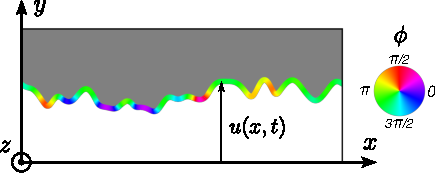
\includegraphics[width=\linewidth]{figuras/snap_system_345.pdf}
    \caption{Snapshot of a DW configuration highlighting its collective coordinates $u(x,t)$ and $\phi(x,t)$. Reproduced from Ref.~\onlinecite{pusiol2026deterministic}.}
\label{fig:snap}
\end{figure}
\rec{Figure 1 caption enhancement: Expand caption to explain the visual elements: ``Snapshot of an extended DW configuration displaying the spatial coordinate $x$ along the wall, the transverse position $u(x,t)$ (solid curve), and the local in-plane magnetization angle $\phi(x,t)$ (arrows and color gradient). Local twists in $\phi$ where the angle rotates by $\pm \pi$ correspond to vertical Bloch lines separating Néel-like segments.''}

Substituting a Bloch domain-wall ansatz
%
\begin{align}
    \theta(x, y, t) &= 2 \arctan\left\{ \exp[{(y - u(x, t))}/{\Delta}] \right\},     \label{eq:Bloch1} \\
    \label{eq:Bloch2}
    \varphi(x, y, t) &= \phi(x, t), 
\end{align}
%
into Eq.~\eqref{eq_LLG}, gives us the reduced coordinate model for the DW. Here $u(x, t)$ and $\phi(x, t)$ represent the local position and the internal magnetization angle of the wall, respectively (see Fig.~\ref{fig:snap}). We assume a constant DW width $\Delta = \sqrt{A_\text{ex}/\left(K_u - \mu_0 M_\text{s}^2/2\right)}$, where the denominator accounts for the effective anisotropy including the magnetostatic demagnetizing energy. 

This model treats the DW as a single-valued directed interface, thereby prohibiting overhangs and loops while allowing for the proliferation and dynamics of vertical Bloch lines. It therefore goes beyond standard elastic interface models by incorporating an internal degree of freedom. We do not consider here the additional effects of thermal fluctuations and quenched disorder.

To simplify the analysis, we nondimensionalize the model using characteristic length, time, and magnetic-field scales~\cite{pusiol2026deterministic}. Distances are measured in units of $u_0 = \Delta$ along the $y$-direction, and $L_0 = \Delta ({2\tilde{K}/N_n})^{1/2}$ in the $x$-direction, where $\tilde{K} = 2 K_u / (\mu_0 M_{s}^2) - 1$. Time is measured in units of $T_0 =(1+\alpha^{2})/(\gamma M_s N_n)$, and the applied field $H_{z}(t)$ is expressed in units of the Walker breakdown field~\cite{skaugen2019} $H_W = \alpha M_s N_n / 2$, with $h(t)=H_{z}(t)/H_{W}$. See Appendix~\ref{ap:exp_cond} for details on the conversion to physical units for a thin Co/Pt multilayer. The resulting equations constitute the $u$--$\phi$ or Slonczewski model~\cite{Slonczewski1972}:
%
\begin{align}
\dot{u} &= \frac{1}{2} \left[ \alpha^2 h(t) + \sin(2\phi) + \alpha \partial_x^2 u - \partial_x^2 \phi \right], \nonumber \\
\dot{\phi} &= \frac{1}{2} \left[ \alpha h(t) - \alpha \sin(2\phi) + \partial_x^2 u + \alpha \partial_x^2 \phi \right].
\label{eq:uphi}
\end{align}
%

This model reduces to the Walker model~\cite{Schryer1974} for rigid DWs, where $\partial ^2_xu=\partial^2_x\phi=0$. To study synchronization phenomena in extended DWs we set $h(t)=h_\text{0}+h_\text{a}\cos\left(\Omega t\right)$, with $h_{0}$ the DC field and $h_{\text{a}}$ the AC field amplitude. Note that the unit of frequency in this system is $1/T_0$. We then numerically solve the full system of coupled, non-autonomous nonlinear partial differential equations using a pseudo-spectral Crank--Nicolson scheme (see Appendix~\ref{ap:num_met} for details).

\section{Synchrony in rigid domain walls}
\label{sec:flat_sync}

Given that the extended DW can become flat under certain conditions, it is relevant to study synchrony in the resulting rigid DW, described by the Walker model. This rigid-DW regime represents the simplest form of macroscopic order the DW can exhibit, and is considerably more analytically tractable than the full extended model.

To simplify the analysis, we define the variables $\tau\equiv\Omega t$, $q(x,\tau)\equiv  u(x,\tau/\Omega)$ and $\psi(x,\tau)\equiv2\phi(x,\tau/\Omega)$. If we assume a spatially uniform DW given by $q(x,\tau)=q_1(\tau)$ and $\psi(x,\tau)=\psi_1(\tau)$, Eqs.~\eqref{eq:uphi} yields the following system of coupled ordinary differential equations for $q_1$ and $\psi_1$:
%
\begin{align}
    \dot{q}_1 &= \frac 1 {2\Omega} \left[ \alpha ^2h_0+\alpha^2h_\text{a}\cos(\tau) + \sin (\psi_1)\right], 
    \label{eq:walker_tau1}
    \\
    \dot \psi_1 &= \frac \alpha \Omega \left[ h_0 +  h_\text{a}\cos(\tau) - \sin(\psi_1) \right],
    \label{eq:walker_tau2}
\end{align}
%
The period of the non-autonomous term is fixed to $2\pi$, and Eq.~\eqref{eq:walker_tau2} depends only on the parameters $h_0$, $h_\text a$ and the ratio $\alpha/\Omega$. We will focus on this equation since it is decoupled from the $q_1$ solution and dictates the overall dynamics of the system.

For the case $h_\text{a}=0$, Eq.~\eqref{eq:walker_tau2} reduces to the Adler equation~\cite{adler1946study}, for which there is an analytical expression for the time average $\langle\dot\psi_1\rangle_\tau$:
%
\begin{equation}
    \langle\dot \psi_1 \rangle_\tau  = \begin{cases} 
0 & \text{if } \left| h_0\right| \leq 1, \\ 
\operatorname{sgn}(h_0)\dfrac \alpha \Omega \sqrt{h_0^2 - 1} & \text{if }\left| h_0\right| >1.
\end{cases}\
    \label{eq:avg_walker}
\end{equation}
%
In addition, the average velocity of $q_{1}$ is given by
%
\begin{equation}
    \langle \dot{q_{1}} \rangle_{\tau} = \frac{\alpha^{2}+1}{2\Omega}h_{0} - \frac{\alpha}{2}\langle\dot \psi_1\rangle_{\tau}.
    \label{eq:dot_q1_avg}
\end{equation}
%
Note that this expression is also true for the \aleadd{center of mass of the} flexible wall model with periodic boundary conditions. Therefore, for the time-independent driving case we obtain
%
\begin{equation}
    \langle\dot q_1 \rangle_\tau  =
    \begin{cases} 
     \dfrac{\alpha^{2}+1}{2\Omega}h_{0} & \text{if} \left| h_0\right| \leq 1 \ , \\ \\
    \dfrac{\alpha^{2}+1}{2\Omega}h_{0}-\dfrac{\alpha^{2}}{2\Omega}\operatorname{sgn}(h_0) \sqrt{h_0^2 - 1} & \text{if }\left| h_0\right| >1 \ .
    \end{cases}\
    \label{eq:avg_q1_cases}
\end{equation}
%

When $h_\text{a}\neq0$, solutions must be found numerically (see Appendix~\ref{ap:num_met}). To determine if a stable periodic solution exists, we recorded the $\psi_1$ variable modulo $2\pi$ at every period of the drive: the system has converged to a stable periodic solution if and only if these values converge to a single equilibrium value $\psi_\text{eq}$, independent of the initial condition.

Synchrony is expected to occur near the values of $h_0$ for which Eq.~\eqref{eq:avg_walker} yields an integer. Figure~\ref{fig:ej_walker} shows example curves of the steady-state average velocities of both $q_{1}$ and $\psi_{1}$ as a function of the DC field $h_0$, with the white regions marking the synchronization steps where $\langle \dot{\psi_{1}} \rangle_{\tau} = n$, and $n =0,1,2$. A Walker-breakdown-like feature repeats in $\langle \dot q_1 \rangle_\tau$ at each frequency-unlocking transition of the internal degree of freedom $\psi_1$. Within each synchronization step, the translational average velocity is
%
\begin{equation}
    \langle\dot q_1 \rangle_\tau  = \dfrac{\alpha^{2}+1}{2\Omega}h_{0}-\dfrac{\alpha}{2}n, \quad h^{n}_{1}\leq h_{0} \leq h^{n}_{2},
\end{equation}
%
with $h^{n}_{1}<h^{n}_{2}$ delimiting the extension of the $n$-th step. Consequently, the DW mobility within a synchronized state is identical to that of the constant-driving-field case below the Walker field ($|h_0|<1$).

These synchronization regions 
\aleadd{
in $\langle \dot \psi_1 \rangle_\tau$} are known as \textit{Shapiro steps}, %mathematically 
%equivalent 
\aleadd{as they are analogous} 
to those \aleadd{predicted and observed} in the I--V curves of driven \aleadd{overdamped} Josephson junctions~\cite{shapiro1963josephson}.
%
\begin{figure}[htbp]
    \centering
    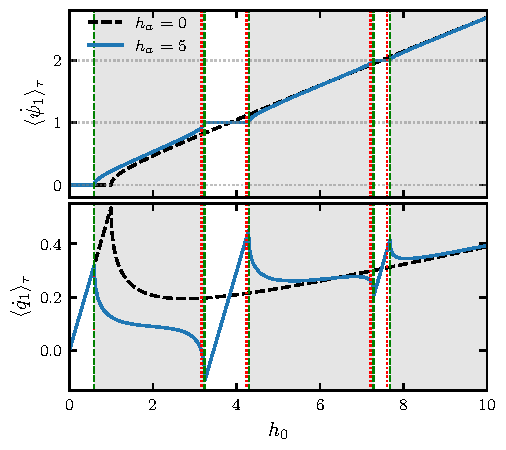
\includegraphics[width=\linewidth]{figuras/figure2.pdf}
    \caption{
    Steady-state average velocities of the internal ($\psi_1$, top) and translational ($q_1$, bottom) degrees of freedom as a function of the DC field $h_0$, for $h_a=0$ (dashed black) and $h_a=5$ (solid blue). White regions indicate the synchronization steps, where $\langle\dot\psi_1\rangle_\tau$ locks to integer multiples of the driving frequency (dotted horizontal lines, top panel). Vertical red dotted lines indicate synchrony boundaries as given by Eq.~\eqref{eq:width_steps}; their second-order approximation, given by Eq.~\eqref{eq:h0_2order}, is shown as green dashed lines. Walker-breakdown-like spikes in $\langle\dot q_1\rangle_\tau$ recur at each unlocking transition of $\psi_1$. 
    }
    \label{fig:ej_walker}
\end{figure}
\rec{Figure 2 suggestions: (i) In the caption, explicitly label panel (a) top and (b) bottom: ``(a) Steady-state average angular velocity $\langle\dot\psi_1\rangle_\tau$ and (b) translational velocity $\langle\dot q_1\rangle_\tau$...'' (ii) In the text, note that within each Shapiro step, the differential mobility $d\langle\dot q_1\rangle_\tau/dh_0 = (\alpha^2+1)/(2\Omega)$ is strictly constant and coincides with the linear sub-Walker mobility, whereas outside the steps the velocity collapses due to chaotic/irregular precession.''}
%
In a synchronized state, solutions should be of the form
%
\begin{equation}
    \psi_\text{s}(\tau) = \psi_\text{c} + n\tau  + \tilde \psi(\tau),
    \label{eq:theta_sync}
\end{equation}
%
with $\psi_\text{c}$ a constant, $\tilde\psi(\tau)$ a $2\pi$-periodic function with zero mean, and $n$ an integer. In this case, it is clear that $\langle \dot\psi_\text{s} \rangle_\tau=n$.

To approximate the boundaries of the parameter regions for which synchronized solutions exist, we can treat the nonlinear $\sin\psi_1$ term as a perturbation by defining the scaled variables $\tilde h_0 \equiv \epsilon h_0$, $\tilde h_\text{a} \equiv \epsilon h_\text{a}$, and introducing $\epsilon \equiv \alpha /\Omega$ as an explicit small parameter. Equation~\eqref{eq:walker_tau2} then reads:
%
\begin{equation}
    \dot{\psi}_1 = \tilde h_0 + \tilde h_\text{a}\cos(\tau) - \epsilon \sin(\psi_1).
    \label{eq:walker_pert}
\end{equation}
%
We now expand both the solution $\psi_1$ and the DC driving parameter $\tilde h_0$ in power series of $\epsilon$:
%
\begin{align}
    \psi_1(\tau) &= \psi^{(0)}(\tau) + \epsilon \psi^{(1)}(\tau) + \epsilon^2 \psi^{(2)}(\tau) + \dots, \\
    \tilde h_0 &= \tilde h_0^{(0)} + \epsilon \tilde h_0^{(1)} + \epsilon^2 \tilde h_0^{(2)} + \dots
    \label{eq:expansion2}
\end{align}
%
Substituting these expansions into Eq.~\eqref{eq:walker_pert} and collecting terms of order $\epsilon^0$, we obtain the unperturbed equation:
%
\begin{equation}
    \dot{\psi}^{(0)} = \tilde h_0^{(0)} + \tilde h_\text{a} \cos(\tau).
\end{equation}

Phase-locking to the $n$-th step requires $\langle \dot{\psi}^{(0)} \rangle_\tau = n$, which fixes $\tilde h_0^{(0)} = n$. Integrating yields the zeroth-order solution:
%
\begin{equation}
    \psi^{(0)}(\tau) = n\tau + \tilde h_\text{a} \sin(\tau) + \psi_\text{c}.
    \label{eq:walker_zeroth}
\end{equation}

At order $\epsilon^1$, the dynamics of the first-order correction $\psi^{(1)}$ are governed by:
%
\begin{equation}
    \dot{\psi}^{(1)} = \tilde h_0^{(1)} - \sin\left(\psi^{(0)}\right).
    \label{eq:dot_psi_1}
\end{equation}
%
For the synchronized solution to remain valid at this order, $\psi^{(1)}$ must remain a $2\pi$-periodic function of zero mean. Therefore, the time average of the right-hand side of Eq.~\eqref{eq:dot_psi_1} must vanish:
%
\begin{equation}
    \tilde h_0^{(1)} = \left\langle \sin\left(\psi^{(0)}\right) \right\rangle_\tau.
\end{equation}
%
Expanding $\sin\left(\psi^{(0)}\right)$ using the Jacobi--Anger identity,
%
\begin{equation}
    \sin\left(\psi^{(0)}\right) = \sum_{m=-\infty}^{\infty}J_{m} (\tilde h_\text{a})\sin[(n+m)\tau+\psi_\text{c}],
\end{equation}
%
we see that every term oscillates with zero mean except the one with $m=-n$. This DC component yields:
%
\begin{equation}
    \tilde h_0^{(1)} = J_{-n}(\tilde h_\text{a})\sin(\psi_\text{c}) = (-1)^{n}J_{n} (\tilde h_\text{a})\sin(\psi_\text{c}).
    \label{eq:firstorder}
\end{equation}
%
Truncating the expansion~\eqref{eq:expansion2} at first order gives $\tilde h_0 \approx n + \epsilon \tilde h_0^{(1)}$. Substituting back the original physical parameters $h_0, h_\text{a}$, $\alpha/\Omega$, and the solution~\eqref{eq:firstorder} for $\tilde h_0^{(1)}$, we obtain:
%
\begin{equation}
    h_{0} \approx \frac{n\Omega}{\alpha} +(-1)^{n}J_{n} \left(\frac{\alpha}{\Omega}h_\text{a}\right)\sin(\psi_\text{c}). 
\end{equation}
%
Since $\sin \psi_\text{c}\in [-1,1]$, a synchronized solution exists only if
%
\begin{equation}
    \left| h_{0} - \frac{n\Omega}{\alpha} \right| \leq \left|J_{n}\left(\frac{\alpha}{\Omega}h_\text{a}\right) \right|.
    \label{eq:walkerwithAC}
\end{equation}
%
Finally, each step is centered at $h_{0}=n\Omega/\alpha$ and has a field-range width 
%
\begin{equation}
    h^{n}_{2}-h^{n}_{1}=2 \left|  J_{n}\left(\frac{\alpha}{\Omega}h_\text{a}\right) \right|.
    \label{eq:width_steps}
\end{equation}


The details of the continuation of this perturbative treatment to second order in $\epsilon$ are worked out in Appendix~\ref{ap:segundo_orden}. The only second order effect is a rigid shift depending only on $\alpha h_\text{a}/\Omega$ in the synchronization steps with $|n|>0$. The correction is more significant for the smaller absolute values of $n$ and $h_\text{a}$, vanishing in the limits where either variable goes to infinity. For the $n=0$ step, the second order corrections vanish identically. \aleadd{In Fig. \ref{fig:ej_walker} we can compare first and second order corrections.}
\rec{Second-order perturbation physical interpretation: Emphasize that the second-order shift $\Delta h_0^{(2)} = \frac{\alpha}{\Omega}A$ arises from the asymmetric time spent by the magnetization vector traversing the attractive versus repulsive quadrants of the nonlinear $\sin(\psi_1)$ torque. Because $A \approx \frac{1}{2n}$ as $h_a \to 0$, this shift is always toward higher DC fields, explaining why numerical Arnold tongues tilt slightly toward larger driving fields for finite damping $\alpha$.}

% In a synchronized state, solutions should be of the form
% \begin{equation}
%     \psi_\text{s}(\tau) =\psi_\text{c}+ n\tau  + \tilde \psi(\tau),
%     \label{eq:theta_sync}
% \end{equation}
% with $\psi_\text{c}$ a constant, $\tilde\psi(\tau)$ a $2\pi$-periodic function with zero mean, and $n$ an integer. In this case, it is clear that $\langle \dot\psi_\text{s} \rangle_\tau=n$.
% It is possible to approximate the boundaries of the parameter regions for which synchronized solutions exist if we treat the nonlinear $\sin\psi_1$ term as a perturbation. If we disregard it, Eq.~\eqref{eq:walker_tau} is trivially integrable \fabricom{with the zeroth-order solution}
% %
% \begin{equation}
% \psi_\text{s,0}(\tau)=n\tau +\psi_\text{c} + \frac{\alpha}{\Omega}h_\text{a} \sin\tau,
%     \label{eq:walker_zeroth}
% \end{equation}
% %   
% \fabricom{with} $\langle\dot\psi_\text{s,0}\rangle_\tau=n\in\mathbb Z$. Now we add a perturbation $\delta\psi(\tau)$, while preserving the form of a synchronized solution \fabricom{[Eq.~\eqref{eq:theta_sync}]}. This implies that $\delta \psi$ must be a $2\pi$-periodic function of zero mean. Substituting $\psi_\text{s,1} = \psi_\text{s,0} + \delta\psi$ into Eq.~\eqref{eq:walker_tau} we find an equation for $\delta\dot\psi$:
% %
% \begin{equation}
%     \delta\dot\psi = \frac \alpha \Omega h_0 -n-\frac \alpha\Omega \sin\left(\psi_\text{s,0} + \delta\psi\right).
%     \label{eq:walker_delta_theta}
% \end{equation}
% %
% \fabricom{
% Since $\delta\psi$ is small, we linearize $\sin\psi_{s,1}$
% \begin{equation}
%     \sin\left(\psi_\text{s,0} + \delta\psi\right)\approx\sin\psi_{s,0}+\delta\psi\cos\psi_{s,0},
% \end{equation}
% leaving a linear, $\tau$-periodically-forced equation for $\delta\psi$
% %
% \begin{equation}
%     \delta\dot\psi = \frac \alpha\Omega [h_0-\sin\psi_{s,0}] - n - \dfrac{\alpha}{\Omega}\delta\psi\cos\psi_{s,0}
%     \label{eq:dot_psi}
% \end{equation}
% %
% The forcing term must have zero mean over one period. Expanding $\sin\psi_{s,0}$ with the Jacobi--Anger identity,
% %
% \begin{equation}
%     \sin\psi_{s,0} = \sum_{m=-\infty}^{\infty}J_{m} \left(\frac{\alpha}{\Omega}h_\text{a} \right)\sin[(n+m)\tau+\psi_{c}],
% \end{equation}
% %
% every term oscillates in $\tau$} \luzcom{with zero mean} \fabricom{except the one with $m=-n$, which is time-independent. Solving for $h_0$, we obtain
% %
% \begin{equation}
%     h_{0} = \frac{n\Omega}{\alpha} +(-1)^{n}J_{n} \left(\frac{\alpha}{\Omega}h_\text{a}\right)\sin\psi_{c}. 
% \end{equation}
% %
% Since $\sin \psi_\text{c}\in [-1,1]$, a synchronized solution exists only if
% %
% \begin{equation}
%     \left| h_{0} - \frac{n\Omega}{\alpha} \right| \leq \left|J_{n}\left(\frac{\alpha}{\Omega}h_\text{a}\right) \right|.
% \end{equation}
% %
% Finally, each step is centered at $h_{0}=n\Omega/\alpha$ and has a field-range width 
% %
% \begin{equation}
%     h^{n}_{2}-h^{n}_{1}=2 \left|  J_{n}\left(\frac{\alpha}{\Omega}h_\text{a}\right) \right|.
%     \label{eq:width_steps}
% \end{equation}
% %
% }
% Stability of Eq.~\eqref{eq:dot_psi} requires
% \begin{equation}
%     \langle \cos\psi_{s,0}(\tau) \rangle=(-1)^{n}J_{n}\left(\frac{\alpha}{\Omega}h_\text{a}\right)\cos\psi_{c}>0.
% \end{equation}
% This condition follows from linearizing Eq.~\eqref{eq:dot_psi} around the fixed point $\delta\psi=0$: since the residual equation for $\delta\psi$ takes the form $\delta\dot\psi \approx -\frac{\alpha}{\Omega}\cos\psi_{s,0}(\tau)\,\delta\psi$ after the zero-mean forcing condition is imposed, its time-averaged coefficient determines whether small perturbations decay or grow. A positive average, $\langle\cos\psi_{s,0}(\tau)\rangle>0$, corresponds to exponential decay of $\delta\psi$ and hence a dynamically stable locked state; a negative average signals an unstable fixed point. Since Eq.~\eqref{eq:theta_sync} admits two solutions for $\psi_\text{c}$ at fixed $h_0$ within each step -- related by $\psi_\text{c}\to\pi-\psi_\text{c}$, which leaves $\sin\psi_\text{c}$ (and thus $h_0$) unchanged while flipping the sign of $\cos\psi_\text{c}$ -- only one of the two is stable.
% }

% \section{Synchrony in rigid domain walls}
% \label{sec:flat_sync}

% Given that the extended \fabricom{DW} can become flat in some conditions, it is relevant to study synchrony in a rigid DW, described by the Walker model. It is also the simplest form of macroscopic order that can be established in the DW, and it is more analytically tractable than the full model. 

% To simplify the analysis, we define the variables \fabricom{$\tau\equiv\Omega t$}, \fabricom{$q(x,\tau)\equiv  u(x,\tau/\Omega)$ and $\psi(x,\tau)\equiv2\phi(x,\tau/\Omega)$}. If we assume a spatially uniform DW given by $q(x,\tau)=q_1(\tau)$ and $\psi(x,\tau)=\psi_1(\tau)$, Eq.~\eqref{eq:uphi} yields the following system of coupled ordinary differential equations for $q_1$ and $\psi_1$:
% %
% \begin{align}
%     \dot{q}_1 &= \frac 1 {2\Omega} \left[ \alpha ^2h_0+\alpha^2h_\text{a}\cos(\tau) + \sin (\psi_1)\right], \\
%     \dot \psi_1 &= \frac \alpha \Omega \left[ h_0 +  h_\text{a}\cos(\tau) - \sin(\psi_1) \right],
%     \label{eq:walker_tau}
% \end{align}
% %
% where the period of the non-autonomous term is fixed to $2\pi$ and the equation for $\psi_1$ depends only on the parameters $h_0$, $h_\text a$ and the ratio $\alpha/\Omega$. We will focus on this equation since it is decoupled from the $q_1$ solution and dictates the overall dynamics of the system. 

% For the case $h_\text{a}=0$, Eq.~\eqref{eq:walker_tau} reduces to the Adler equation\fabricom{[ref]}, for which there is an analytical expression for the time average $\langle\dot\psi\rangle_\tau$:
% %
% \begin{equation}
%     \langle\dot \psi_1 \rangle_\tau  = \begin{cases} 
% 0 & \text{if } \left| h_0\right| \leq 1, \\ 
% \operatorname{sgn}(h_0)\dfrac \alpha \Omega \sqrt{h_0^2 - 1} & \text{if }\left| h_0\right| >1.
% \end{cases}\
%     \label{eq:avg_walker}
% \end{equation}
% %
% \fabricom{In addition, the average velocity of $q_{1}$ is given by
% %
% \begin{equation}
%     \langle \dot{q_{1}} \rangle_{\tau} = \frac{\alpha^{2}+1}{2\Omega}h_{0} - \frac{\alpha}{2}\langle\dot \psi_1\rangle_{\tau},
%     \label{eq:dot_q1_avg}
% \end{equation}
% %
% therefore, for the time-independent driving case we obtain
% %
% \begin{equation}
%     \langle\dot q_1 \rangle_\tau  =
%     \begin{cases} 
%      \dfrac{\alpha^{2}+1}{2\Omega}h_{0} & \text{if} \left| h_0\right| \leq 1 \ , \\ \\
%     \dfrac{\alpha^{2}+1}{2\Omega}h_{0}-\dfrac{\alpha^{2}}{2\Omega}\operatorname{sgn}(h_0) \sqrt{h_0^2 - 1} & \text{if }\left| h_0\right| >1 \ .
%     \end{cases}\
%     \label{eq:avg_q1_cases}
% \end{equation}
% %
% }

% When $h_\text{a}\neq0$, solutions \fabricom{Eq.~\eqref{eq:walker_tau}} must be found numerically. \fabricom{Synchrony is expected to occur near the values of $h_0$ for which Eq.~\eqref{eq:avg_walker} yields an integer}. \fabricom{Figure~\ref{fig:ej_walker} shows example curves of the steady-state average velocities of both $q_{1}$ and $\psi_{1}$ as a function of the DC field $h_0$, with the grey shaded regions marking the synchronization steps where $\langle \dot{\psi_{1}} \rangle_{\tau} = n$, and $n =0,1,2$. A Walker-breakdown like feature repeats in $\langle \dot q_1 \rangle_\tau$ at each frequency-unlocking transition of the internal degree of freedom $\psi_1$. Within each synchronization step, the translational average velocity is
% %
% \begin{equation}
%     \langle\dot q_1 \rangle_\tau  = \dfrac{\alpha^{2}+1}{2\Omega}h_{0}-\dfrac{\alpha}{2}n, \quad h^{n}_{1}\leq h_{0} \leq h^{n}_{2},
% \end{equation}
% %
% with $h^{n}_{1}<h^{n}_{2}$ delimiting the extension of the $n$-th step. Then, the DW mobility of a synchronized solution is the same as the constant driving field case below the Walker field ($\vert h_{0}\vert<1$).

% These synchronization regions are known as \textit{Shapiro steps}, mathematically equivalent to those observed in the I-V curves in driven Josephson junctions~\cite{shapiro1963josephson}.
% }


% In a synchronized state, solutions should be of the form
% \begin{equation}
%     \psi_\text{s}(\tau) =\psi_\text{c}+ n\tau  + \tilde \psi(\tau),
%     \label{eq:theta_sync}
% \end{equation}
% with $\psi_\text{c}$ a constant, $\tilde\psi(\tau)$ a $2\pi$-periodic function with zero mean, and $n$ an integer. In this case, it is clear that $\langle \dot\psi_\text{s} \rangle_\tau=n$.
% It is possible to approximate the boundaries of the parameter regions for which synchronized solutions exist if we treat the nonlinear $\sin\psi_1$ term as a perturbation. If we disregard it, Eq.~\eqref{eq:walker_tau} is trivially integrable \fabricom{with the zero-order solution}
% %
% \begin{equation}
% \psi_\text{s,0}(\tau)=n\tau +\psi_\text{c} + \frac{\alpha}{\Omega}h_\text{a} \sin\tau,
%     \label{eq:walker_zeroth}
% \end{equation}
% %   
% \fabricom{with} $\langle\dot\psi_\text{s,0}\rangle_\tau=n\in\mathbb Z$. Now we add a perturbation $\delta\psi(\tau)$, while preserving the form of a synchronized solution \fabricom{[Eq. ~\eqref{eq:theta_sync}]}. This implies that $\delta \psi$ must be a $2\pi$-periodic function of zero mean. Substituting $\psi_\text{s,1} = \psi_\text{s,0} + \delta\psi$ into Eq.~\eqref{eq:walker_tau} we find an equation for $\delta\dot\psi$:
% %
% \begin{equation}
%     \delta\dot\psi = \frac \alpha \Omega h_0 -n-\frac \alpha\Omega \sin\left(\psi_\text{s,0} + \delta\psi\right).
%     \label{eq:walker_delta_theta}
% \end{equation}
% %
% \fabricom{
% Since $\delta\psi$ is small, we linearize $\sin\psi_{s,1}$
% \begin{equation}
%     \sin\left(\psi_\text{s,0} + \delta\psi\right)\approx\sin\psi_{s,0}+\delta\psi\cos\psi_{s,0},
% \end{equation}
% leaving a linear, $\tau$-periodically-forced equation for $\delta\psi$
% %
% \begin{equation}
%     \delta\dot\psi = \frac \alpha\Omega [h_0-\sin\psi_{s,0}] - n - \dfrac{\alpha}{\Omega}\delta\psi\cos\psi_{s,0}
%     \label{eq:dot_psi}
% \end{equation}
% %
% The forcing term must have zero mean, therefore, expanding $\sin\psi_{s,0}$ with the Jacobi–Anger identity
% %
% \begin{equation}
%     \sin\psi_{s,0} = \sum_{m=-\infty}^{\infty}J_{m} \left(\frac{\alpha}{\Omega}h_\text{a} \right)\sin[(n+m)\tau+\psi_{c}],
% \end{equation}
% %
% every term oscillates in $\tau$, except the $m=-n$ which is time-independent. Solving for $h_{0}$ we obtain,
% %
% \begin{equation}
%     h_{0} = \frac{n\Omega}{\alpha} +(-1)^{n}J_{n} \left(\frac{\alpha}{\Omega}h_\text{a}\right)\sin\psi_{c}. 
% \end{equation}
% %
% Since $\sin \psi_\text{c}\in [-1,1]$, a synchronized solution exists only if
% %
% \begin{equation}
%     \left| h_{0} - \frac{n\Omega}{\alpha} \right| \leq \left|J_{n}\left(\frac{\alpha}{\Omega}h_\text{a}\right) \right|.
% \end{equation}
% %
% Finally, each step is centered at $h_{0}=n\Omega/\alpha$ and a field-range width 
% %
% \begin{equation}
%     h^{n}_{2}-h^{n}_{1}=2 \left|  J_{n}\left(\frac{\alpha}{\Omega}h_\text{a}\right) \right|.
% \end{equation}
% %

% Stability of Eq.~\ref{eq:dot_psi} requires
% \begin{equation}
%     \langle \cos\psi_{s,0}(\tau) \rangle=(-1)^{n}J_{n}\left(\frac{\alpha}{\Omega}h_\text{a}\right)\cos\psi_{c}>0
% \end{equation}
% }

%The Walker field in the absence of AC driving ($h_{0}=1$) is reduced when the AC field is turned on (No estoy seguro de esto)
% Rigid wall dynamics. Comparison of average velocity curves for both the $\psi_1$ and $q_1$ variables as a function of the DC field $h_0$, for AC fields $h_\text{a}$ of 0 and 5, with $\alpha=0.27$ and $\Omega=1$. Synchronization steps are highlighted.}
% Given that the perturbation is of order $\alpha/\Omega$, we can neglect $\delta\psi$ in the sine term of Eq.~\eqref{eq:walker_delta_theta}
% Since $\delta \psi$ is periodic and has a mean of zero, its derivative also has zero mean. We then use the Jacobi-Anger expansion in terms of Bessel functions of the first kind:
% \begin{equation}
% \sin\left(x+z\sin y\right) = \sum_{m=-\infty} ^\infty J_m(z) \sin\left(x+my\right) \ .
%     \label{eq:jacobi-anger}
% \end{equation}

% By substituting $\psi_\text{s,0}$ into Eq.~\eqref{eq:walker_delta_theta}, and applying the expansion with $x=n\tau+ \psi_\text{c}$, $y=\tau$ and $z=\frac \alpha \Omega h_\text{a}$, the zero-mean condition yields:

% \begin{equation}
% 0=\frac \alpha\Omega h_0 -n - \frac \alpha \Omega \sum_{m=-\infty}^\infty J_m\left(\frac \alpha \Omega h_\text{a}\right)\left\langle{\sin\left(\psi_\text{c} + (n+m)\tau \right)}\right\rangle_\tau \ .
%     \label{eq:walker_jacobi}
% \end{equation}

% The only non-zero term in the series corresponds to $m=-n$. We can solve for $h_0$:
% \begin{equation}
% h_0 = \frac \Omega \alpha n + J_{-n}\left(\frac \alpha \Omega h_\text{a}\right)\sin\psi_\text{c} \ .
% \label{eq:walker_steps}
% \end{equation}

% From this equation we can conclude that the centers of the synchronization steps are evenly spaced, and that the spacing grows linearly with the driving frequency $\Omega$. Since $\sin \psi_\text{c}\in [-1,1]$ and $J_{-n}(z) =(-1)^n J_{n}(z)$, the width $\Delta_n$ of a given step is given by

% \begin{equation}
%  \Delta_n = 2\left|J_n\left(\frac \alpha \Omega h_\text{a} \right)\right| \ .
%     \label{eq:walker_step_width}
% \end{equation}


% \luzcom{No sé si esta parte de la estabilidad de las soluciones sincronizadas en el modelo de Walker es muy relevante. Tal vez mejor saltar directamente a (*)}
% To see if the periodic solutions are stable, we can introduce a small perturbation $\delta\psi$ to a solution of the form~\eqref{eq:theta_sync}. Substituting into Eq.~\eqref{eq:walker_tau} and linearizing $\sin\left(\psi_\text {s}+\delta\psi\right)\approx \sin\left(\psi_\text {s}\right) + \cos\left(\psi_\text {s} \right) \delta \psi$, the first order linear ordinary differential equation for the perturbation is:
% \begin{equation}
%     \delta\dot\psi = -\frac \alpha \Omega \cos\psi_\text{s} \, \delta\psi \ .
%     \label{eq:walker_perturbation}
% \end{equation}

% Noting that $\cos\psi_\text{s}$ is $2\pi$-periodic, we can apply Floquet theory. The solution can be written as $\delta\psi = \exp(R \tau)P(\tau)$, with $P$ a $2\pi$-periodic function and

% \begin{equation}
%     R = \frac 1 {2\pi} \int_{0}^{2\pi}\!\!\!\! -\frac \alpha \Omega \cos\left(\psi_\text{s}(\tau)\right)\mathrm d\tau=-\frac \alpha \Omega\left\langle \cos \left(\psi_\text{s}(\tau)\right)\right\rangle_\tau\ .
%     \label{eq:walker_floquet}
% \end{equation}

% As the periodic factor is necessarily bounded, the stability of the synchronized solution is determined by the sign of $\langle\cos\left(\psi_\text{s}(\tau)\right)\rangle_\tau$. If it is negative, the perturbation grows exponentially. If it is positive, then the perturbations decay and the synchronized state is stable. This is useful as a numerical tool to ensure that the periodic solutions found are actually stable. 
% \luzcom{(*)}

\section{Linear stability of flat, synchronized domain walls}
\label{sec:linearstabilitydiagrams}

To study the linear stability of synchronized flat solutions, we adopt the theoretical framework recently detailed by Pusiol et al.~\cite{pusiol2026deterministic} and extend it to account for a time-dependent magnetic field. We linearize a solution of Eq.~\eqref{eq:uphi} $\mathbf{v}(x,\tau)\equiv(u,\phi)^{T}$ around the flat-wall solution,
%
\begin{equation}
    \mathbf{v}(x,\tau) = \mathbf{v}_{1}(\tau) + \boldsymbol{\eta}(x,\tau), \quad \boldsymbol{\eta}(x,t) \equiv \begin{pmatrix} Q(x,t) \\ \Phi(x,t) \end{pmatrix}
\end{equation}
%
where $\mathbf{v}_{1}(\tau)\equiv(q_{1}(\tau),\psi_1(\tau)/2)^{T}$. Substituting into Eq.~\eqref{eq:uphi}, the linearized system reads
%
\begin{equation}
    \partial_\tau \boldsymbol{\eta} = \frac{1}{2\Omega}\,\mathcal{M}(\tau)\,\boldsymbol{\eta},
    \label{eq:linearized_matrix}
\end{equation}
%
with
%
\begin{equation}
    \mathcal{M}(\tau) \equiv
    \begin{pmatrix}
    \alpha\,\partial_x^2 & -\partial_x^2+2\cos\psi_1(\tau) \\
    \partial_x^2 & \alpha\,\partial_x^2-2\alpha\cos\psi_1(\tau)
    \end{pmatrix}.
    \label{eq:stability_matrix}
\end{equation}
%
We perform a Fourier transform in space, so that $\partial_x^2\to-\kappa^2$. Since Eq.~\eqref{eq:linearized_matrix} is linear with $x$-independent coefficients, distinct modes $\kappa$ decouple, yielding
%
\begin{equation}
    \partial_\tau \boldsymbol{\eta}_\kappa = \frac{1}{2\Omega}\,\mathcal{M}_\kappa(\tau)\,\boldsymbol{\eta}_\kappa,
    \label{eq:linearized_mode}
\end{equation}
%
with
%
\begin{equation}
    \mathcal{M}_\kappa(\tau) \equiv -\kappa^2
    \begin{pmatrix}
    \alpha & -1 \\
    1 & \alpha
    \end{pmatrix}
    + 2\cos\psi_1(\tau)
    \begin{pmatrix}
    0 & 1 \\
    0 & -\alpha
    \end{pmatrix},
    \label{eq:stability_matrix_split}
\end{equation}
%
where the first term is the $\tau$-independent diffusive coupling between $Q_\kappa$ and $\Phi_\kappa$, and the second is the $2\pi$-periodic modulation set by the rigid-wall background solution $\psi_1(\tau)$. The stability of a linear system with periodic coefficients can be determined using Floquet theory. By Floquet's theorem, a general solution of Eq.~\eqref{eq:linearized_mode} can be written as
%
\begin{equation}
    \boldsymbol{\eta}_{\kappa}(\tau) = P_\kappa(\tau)\,e^{R_\kappa\tau}\,\boldsymbol{\eta}_\kappa(0),
\end{equation}
%
where $P_\kappa(\tau)$ is a $2\pi$-periodic matrix and $R_\kappa$ is a constant matrix. The monodromy matrix $M_\kappa \equiv P_\kappa(2\pi)\,e^{2\pi R_\kappa}$ is obtained by integrating Eq.~\eqref{eq:linearized_mode} over one period, using the canonical initial conditions $\boldsymbol{\eta}_\kappa(0) = (1,0)^T$ and $(0,1)^T$. The amplitude of the perturbation grows exponentially -- indicating that the system is unstable -- whenever the Floquet multiplier (eigenvalue of $M_\kappa$) of largest modulus, $\mu_\kappa$, satisfies $|\mu_\kappa|>1$. Since the modes $\kappa$ are decoupled, their Floquet multipliers can be computed independently, allowing straightforward parallelization across $\kappa$. Furthermore, the rescaled time conveniently fixes the integration interval to $2\pi$ regardless of parameter values.
\rec{Connection to Growth Rates and Hill Expansion: State explicitly that the continuous mode growth rate is $\lambda_\kappa = \frac{\Omega}{2\pi}\ln|\mu_\kappa|$. Modes with $\operatorname{Re}(\lambda_\kappa)>0$ grow exponentially. This directly connects the numerical monodromy calculation to the analytical multi-harmonic Hill matrix expansion detailed in the Supporting Information (see Appendix E), where the eigenvalues of the secular matrix $\mathcal{H}(\kappa)$ yield $\lambda_\kappa$ algebraically.}

% \begin{align}
%     \dot{q}_{1} &= \dfrac{1}{2\Omega}\left[\alpha^{2} h_0+\alpha^2h_\text{a}\cos\left(\tau\right) + \sin(\psi_{1}(\tau))\right], \\
% \dot{\psi}_{1} &= \dfrac{\alpha}{\Omega}\left[h_0 +  h_\text{a}\cos\left(\tau\right) - \sin( \psi_1(\tau))\right].
% \end{align}
% If $\Phi \ll 1$ (no assumption is made regarding $Q$), $\sin(2\tilde\phi) \approx \sin(\psi_1)+ 2 \cos(\psi_1) \Phi$. Then, 
% \begin{align}
%     \partial_\tau Q &=  \frac{\cos(\psi_1)}{\Omega} \Phi + 
%     \frac{1}{2\Omega}(\alpha \partial_x^2Q-\partial_x^2\Phi) \ ,
%     \\
% \partial_\tau \Phi &= - \frac{\alpha}{\Omega} \cos(\psi_1) \Phi +
% \frac{1}{2\Omega}(\partial_x^2Q+ \alpha \partial_x^2\Phi)\ . 
% \label{eq:lineardynamics}
% \end{align}
% To decouple the linear system we use spatial Fourier transform: $Q(x,t)\mapsto\hat{Q}_\kappa(t)$, $\Phi(x,t)\mapsto\hat{\Phi}_\kappa(t)$, where $\kappa$ denotes a mode wavevector in units of $1/L_{0}$. For each mode, we obtain a $2\times2$ linear system as follows:
% \begin{equation}
%     \partial_\tau \begin{pmatrix}
%         \hat Q_\kappa\\
%         \hat \Phi_\kappa
%     \end{pmatrix} =\frac 1 \Omega \begin{pmatrix}
%         -\alpha\frac{\kappa^2}{2} & \frac{\kappa^2}{2}+\cos(\psi_1(\tau))\\
%         -\frac{\kappa^2}{2} & -\alpha\left(\frac{\kappa^2}{2} +\cos(\psi_1(\tau)) \right)
%     \end{pmatrix}
%     \begin{pmatrix}
%         \hat Q_\kappa \\ \hat \Phi_\kappa
%     \end{pmatrix} \ .
%     \label{eq:sistema_linealizado}
% \end{equation}
% If $\psi_1$ is a synchronized rigid wall solution $\psi_\text{s}$, its cosine is $2\pi$-periodic. This enables us to use Floquet theory to analyze the stability of the rigid wall. Floquet's theorem states that the general solution can be written as

% \begin{equation}
%     \begin{pmatrix}
%         \hat{Q}_\kappa(\tau)\\
%         \hat{\Phi}_\kappa(\tau)
%     \end{pmatrix}
%  = P(\tau) e^{R \tau}     
%  \begin{pmatrix}
%         \hat{Q}_\kappa(0)\\
%         \hat{\Phi}_\kappa(0)
%     \end{pmatrix},
%     \label{eq:floquet}
% \end{equation}
% where $P(\tau)$ is a $2\pi$-periodic matrix function and $R$ a constant matrix. The monodromy matrix $M_\kappa \equiv P(2\pi ) \, e^{2\pi R}$ is obtained by integrating the system \eqref{eq:sistema_linealizado} over one period with initial conditions $(\hat Q_{\kappa}(0), \hat \Phi_{\kappa}(0)) = (1, 0)$ and $(0, 1)$. The first solution yields the first column of $M_\kappa$, and the second solution forms the second column. Evaluating \eqref{eq:floquetsys} at integer multiples of $2\pi$ gives
% \begin{equation}
%  \begin{pmatrix}
%         \hat{Q}_\kappa(2 \pi n)\\
%         \hat{\Phi}_\kappa(2 \pi n)
%     \end{pmatrix}    
% = M_\kappa^n 
% \begin{pmatrix}
%         \hat{Q}_\kappa(0)\\
%         \hat{\Phi}_\kappa(0)
%     \end{pmatrix}.
% \end{equation}

% The amplitude of the perturbations grows exponentially if the largest eigenvalue $\mu_\kappa$ of $M_\kappa$, or Floquet multiplier, satisfies $\left| \mu_\kappa \right|>1$, which implies the system is unstable. 

% Floquet multipliers can be easily computed in parallel since the modes are decoupled. Furthermore, the normalization of the time scale $\Omega t \mapsto \tau$ conveniently fixes the integration interval to $2\pi$ for all parameter values.

% We emphasize that this analysis is only valid for those combinations of $h_0$, $h_\text{a}$ and $\alpha/\Omega$ for which the rigid wall equations have a stable periodic solution. For this reason it is useful to map those regions in the parameter space in order to link synchrony and macroscopic spatial order. Additionally, the rigid wall state is not the only possible way for stable collective spatial order to occur, and we have observed that synchrony can induce order with a different spatial dependence. 

% First we define a scaled time $\tau=\Omega t$, and the variables $q(x,\tau)=u(x,\tau/\Omega)$ and $\tilde \phi=\phi(x,\tau/\Omega)$. Then

% \begin{align}
% q(x, \tau) &= Q \left(x,\tau \right)+q_{1}(\tau), \\
% \tilde \phi(x, \tau) &= \Phi\left(x,\tau \right)+\psi_{1}(\tau)/2, 
% \end{align}
% \section{Numerical Results}
% \subsection{Linear stability of 
% \alecom{flat}
%rigid 
%synchronized DWs}

\begin{figure}[htbp]
    \centering
    \begin{overpic}[width=\linewidth]{figuras/figure3.pdf}
        \put(14, 90){\textbf{(a)} $h_\mathrm{a}=2$}
        \put(14, 46){\textbf{(b)} $h_\mathrm{a}=3$}
    \end{overpic}
    \caption{
    Linear stability diagram of DW modes for $\alpha=0.27$ and $\Omega = 1$, with $h_\text{a} = 2$ in (a) and $h_\text{a}=3$ in (b). White regions are stable; gray regions do not admit a stable time-periodic solution for the rigid wall. Color indicates the magnitude of the largest Floquet multiplier for unstable regions with $\left|\mu_\kappa\right|>1$.
    }
    \label{fig:sync_stability}
\end{figure}

Figure~\ref{fig:sync_stability} shows the resulting stability diagrams obtained numerically for $h_a=2$ (a) and $h_a=3$ (b), at $\alpha=0.27$ and $\Omega=1$, as an illustrative example. Although the rigid DW is synchronized within the corresponding Shapiro steps, finite intervals of $h_0$ exhibit spatial instabilities. These unstable regions are generally located near the boundaries of the synchronization steps and are characterized by a finite range of wavenumbers with Floquet multipliers satisfying $|\mu_\kappa|>1$. Thus, synchronization of the internal precessional dynamics if the rigid DW does not necessarily imply spatial stability of the extended flexible DW. Instead, a synchronized flat DW can coexist with a band of unstable spatial modes, whose growth rates depend continuously on $\kappa$. The nonlinear evolution of these instabilities, \aleadd{and also the possible instabilities of non synchronized flat walls (for which Floquet analysis is not adapted)}, and their effect on the long-time DW structure are investigated in the following section.
\rec{Figure 3 Discussion \& Typo: (i) Fix typo: ``internal precessional dynamics if the rigid DW'' $\to$ ``internal precessional dynamics of the rigid DW''. (ii) Physical explanation of Fig.~3 features: Highlight that the instability bands (colored tongues) are parametric resonances occurring near $\kappa^2 \approx m\Omega$. For $h_a=2$ (weak drive), individual tongues corresponding to $m=0, 1, 2$ are well-separated. For $h_a=3$ (stronger drive), inter-channel coupling hybridizes adjacent resonances, opening a reentrant stable region (a ``waist'') where the flat synchronized wall is restored. This non-monotonic stability window directly determines the morphology of the dynamical phase diagram.}


% Figure~\ref{fig:walker_sync} shows a map of the regions or Arnold tongues~\cite{Pikovsky_Rosenblum_Kurths_2001}, for which the rigid DW equations, Eqs.~\eqref{eq:walker_tau}, have a synchronized solution as a function of $h_0$ and $h_\text{a}$ for $\alpha = 0.27$ and $\Omega = 1$, as well as whether they are linearly stable in the extended DW model. The gray regions do not admit a time-periodic solution. White indicates that the time-periodic rigid DW solution is also stable. Color indicates the maximum Floquet multiplier across all wavenumbers in the cases for which the periodic solution is not stable. Dashed lines outline the boundaries of the stability region as given by the small-nonlinearity approximation \eqref{eq:walker_steps}. The approximation is in good agreement with the exact results, especially for the zeroth synchrony step and for high $h_\text{a}$ values. Fig.~\ref{fig:sync_stability} shows the full stability diagram for $h_\text{a} =2.15$ (a) and $h_\text{a} = 4$ (b), both of which display instabilities for some values of $h_0$. Instability regions are generally found to be located near the edges of a synchrony region.

% Figure~\ref{fig:walker_sync} illustrates the parameter combinations for which we expect the synchronized, rigid DW to be unstable in the thermodynamic limit of large system sizes. For those systems, the large density of modes ensures that many of them lie in an unstable interval. For smaller systems, finite-size effects are relevant. If the system size is small enough, its available modes may all lie outside the instability interval. In this case, the finite-size wall remains flat.



%\aleadd{
% \section{Nonlinear dynamics of extended DWs}



% We now investigate the long-time dynamics under the combined DC+AC field, going beyond the linear stability analysis of rigid synchronized states. As an illustrative example, we numerically simulate the system of Eqs.~\eqref{eq:uphi} (see Appendix \ref{ap:num_met}) over a range of $h_0$ and $h_\text{a}$, with fixed $\alpha=0.27$ and $\Omega=1$, and characterize the resulting dynamics through the mean angular velocity $\langle\dot\phi\rangle_{x,t}$, the mean DW velocity $\langle\dot u\rangle_{x,t}$, and the roughness
% %
% \begin{equation}
% \langle w^2\rangle_t =
% \left\langle
% \left\langle u^2\right\rangle_x
% -\left\langle u\right\rangle_x^2
% \right\rangle_t .
% \end{equation}
% %
% The time averages are taken after the system has reached its long-time dynamical regime. We characterize synchronization with the external drive through the quantity
% %
% \begin{equation}
% \sigma =
% \left|
% \frac{\left\langle\dot\phi\right\rangle_{x,t}}{\Omega/2}
% -
% \operatorname{round}
% \left(
% \frac{\left\langle\dot\phi\right\rangle_{x,t}}{\Omega/2}
% \right)
% \right|,
% \label{eq:sigma}
% \end{equation}
% %
% which measures the distance of the mean precessional frequency from the nearest integer multiple of $\Omega/2$. Since the nonlinearity depends on $2\phi$, synchronized states lock to frequencies that are integer multiples of $\Omega/2$, giving $\sigma=0$. In practice, for numerical calculations we therefore use $\sigma < \sigma_{\rm tol}$ as the criterion for synchronization, for a given small enough tolerance $\sigma_{\rm tol}$ controlling the precision of Shapiro steps location. 
% %\alecom{$\sigma=0$ o $\sigma<\epsilon$ con alguna tolerancia?}.

% To highlight finite size effects, we consider both a small system with $L/L_0=7$, for which the first nonzero mode is $\kappa=2\pi/7$, and a large system with $L/L_0=1000$. The latter exhibits deterministic spatiotemporal chaos under a purely DC drive in a finite range of $1 < h_0 < h_c$ above the corresponding critical field $h_c \approx $ \alecom{Fabri?}, while the former \alecom{Fabri?}
% % , with all fields normalized by the Walker field $h_W$
% ~\cite{pusiol2026deterministic}. 

% Figure~\ref{fig:wall_metrics} summarizes the response of these extended walls for a fixed AC amplitude $h_\text{a}=3$. Panel (a) shows the absolute value of the Floquet multiplier for the mode $\kappa=2\pi/7$, available only for the flat DW Shapiro steps, as a function of $h_0$. Panels (b)--(d) show the corresponding mean DW velocity, mean angular velocity, and roughness for the two system sizes, together with the rigid-wall result for comparison. In all the plots white/gray regions correspond to synchronized/unsynchronized flat DW solutions. 

% Both systems present synchronization steps in the steady-state precession velocity $\langle \dot \phi \rangle_{x,t}$, and 
% a Walker breakdown alike structure near all synchronization edges, but also display complex features with marked differences with the rigid wall behavior for the same parameters (indicated with the dashed line), and differences between them. Figure~\ref{fig:wall_metrics}(b) shows a large departure of the large DW with respect to the rigid DW near and oustide the Shapiro steps seen in Figure~\ref{fig:wall_metrics}(c), while the small DW displays $h$ windows where the DW velocity is indistinguishable from the rigid wall. This behaviour is strongly correlated with the roughness of the DWs in Figure~\ref{fig:wall_metrics}(d). While the large DW presents a large roughness except in a few small windows, the short DW present a smaller roughness and wider windows of flatness which are concomitant with the rigid wall behavior. 



% While outside the rigid DW synchronization steps we can no apply Floquet theory, the nonlinear dynamics within synchronization steps can be directly correlated with the linear stability structure of flexural modes, such as the one illustrated in Fig. \ref{fig:sync_stability}. When all spatial modes of a synchronized rigid DW are linearly stable, the system evolves toward and remains in the corresponding rigid synchronized state. In this regime, temporal synchronization is accompanied by spatial ordering of the wall into a flat configuration. Importantly, this synchronized flat state can occur for values of $h_0$ that are unstable in the purely DC-driven system~\cite{pusiol2026deterministic}. Thus, the AC drive can restore the stability of the flat DW while simultaneously locking its precessional dynamics to the external drive. This correlation between linear stability and non-linear dynamics is better appreciated by comparing the fundamental mode Floquet multiplier in the white ranges in Figure~\ref{fig:wall_metrics}(a), with the corresponding steady-state roughness in Figure~\ref{fig:wall_metrics}(d). This is so because the instability of the short DW is strictly driven by the its first mode, while for the large system there is a band of linearly instable modes.

% In summary, when a synchronized flat state contains linearly unstable modes, the initially flat configuration becomes corrugated if the system size permits an unstable mode. The resulting nonlinear state need not lose temporal synchronization: the spatial instability can coexist with frequency locking. As illustrated in Fig.~\ref{fig:wall_metrics}, the extended DWs can therefore exhibit both flat and corrugated synchronized states, as well as flat states without synchronization. The corrugated synchronized state, whose roughness is finite but significantly smaller than the one in the chaotic regime, will be analyzed in detail below, where we describe and characterize all possible dynamical phases in a DC+AC amplitudes phase diagram, for a fixed AC frequency.
% % to determine whether the temporal and spatial order persist in the long-time limit.
% }
% % \subsection{Nonlinear dynamics of extended DWs}

% % \aleadd{We now discuss the steady-states under the DC+AC field, going beyond the linear stability analysis done exclusively for rigid synchronized states.}
% % To this end, we simulate the system for a range of $h_0$ and $h_\text{a}$ values, with fixed $\alpha=0.27$ and $\Omega = 1$, and record the mean angular velocity $\langle \dot \phi \rangle_{x,t}$, mean $u$ velocity $\langle\dot u\rangle_{x,t}$, and roughness\begin{equation}
% %       \langle w ^2\rangle_t = \left\langle \left\langle u^2 \right \rangle_x- \left \langle u \right \rangle_x ^2 \right\rangle_t .
% % \end{equation} The time averages are taken after the DW has settled into a steady state. We measure the synchrony with the drive via a quantity $\sigma$, defined as the distance to the nearest integer of $\langle\dot\phi\rangle_{x,t}/\left(\Omega/2\right)$:\begin{equation}
% %     \sigma = \left|\frac{\left\langle \dot \phi \right\rangle_{x,t}}{\Omega/2} -\operatorname{round}\left(\frac{ \left\langle \dot \phi \right \rangle_{x,t}}{\Omega/2} \right) \right| \, .
% %     \label{eq:sigma}
% % \end{equation} Since the nonlinearity depends on $2\phi$, in synchrony the system locks to an angular frequency which is an integer multiple of $\Omega/2$. In this condition, $\sigma=0$, which allows us to define a criterion for synchrony.

% % We perform this analysis for a small system of $L/L_0 = 7$, which has a single unstable mode at $\kappa \approx 0.9$, and for a large system of $L/L_0=1000$ for which the DW displays deterministic spatiotemporal chaos with a purely DC drive. 

% % Figure~\ref{fig:wall_metrics}(a) shows the absolute value of Floquet multipliers for wavenumber $\kappa=2\pi/7$, which is the first non-zero mode for the wall of length $7$, for a fixed $h_\text{a}=3$. Figs.~\ref{fig:wall_metrics}(b)--\ref{fig:wall_metrics}(d) show how the instabilities are reflected in the DW collective behavior, displaying $\langle \dot u\rangle_{x,t}$, $\langle \dot \phi\rangle_{x,t}$ and $\langle w^2\rangle_t$. This particular configuration exhibits a rich variety of behaviors. Both sizes of DW can become flat with or without synchrony, and both can exhibit a synchronized but rough state. 




% % % \subsubsection{Linearly stable synchronized flat DWs}
% % In the cases in which all modes \aleadd{of a synchronized flat DW} are linearly stable, the system evolves into and remains in a rigid wall synchronized state. In this regime, temporal order induces spatial order in the form of a flat solution. Note that this \alecom{may} happen for values of $h_0$ which had unstable modes without AC driving~\cite{pusiol2026deterministic}. \aleadd{Therefore, for such values of the DC field $h_0$, the addition of the AC field can restabilize the flat solution and sync it to the external AC field}.
% %  \fabriq{Acá hay que aclarar/mostrar que sin AC driving $h_{c}\approx7$ para $\alpha=0.27$, porque esto no está demostrado en este trabajo, pero si en Ref.~\cite{pusiol2026deterministic}.} 

% % % \subsubsection{Linearly unstable synchronized flat DWs}
% % The unstable modes lead to a breakdown of the initially flat wall, as with the purely DC-driven case, and cause corrugation to occur if the system size allows a mode in the unstable region. It is worth investigating whether spatial or temporal order is broken due to the linearly unstable modes.  


\aleadd{
\section{Nonlinear dynamics of extended DWs}\label{sec:nonlinear}

We now investigate the long-time dynamics under the combined DC+AC field, going beyond the linear stability analysis of rigid synchronized states. As an illustrative example, we numerically simulate the system of Eqs.~\eqref{eq:uphi} (see Appendix~\ref{ap:num_met}) for the same parameters of the stability map of Fig. \ref{fig:sync_stability}(b). We characterize the resulting dynamics through the mean angular velocity $\langle\dot\phi\rangle_{x,t}$, the mean DW velocity $\langle\dot u\rangle_{x,t}$, and the roughness
%
\begin{equation}
\langle w^2\rangle_t =
\left\langle
\left\langle u^2\right\rangle_x
-\left\langle u\right\rangle_x^2
\right\rangle_t .
\label{eq:roughnessvst}
\end{equation}
%
The time averages are taken after the system has reached its long-time dynamical regime.}

\luzcom{
We characterize synchronization with the external drive through the quantity $\left\langle \sigma^2\right\rangle_x$ by sampling the displacement of the DW $u(x,t+2T_\text{drive})-u(x,t)$ stroboscopically, at intervals of twice the period of the drive $T_\text{drive}=2\pi/\Omega$. For each point on the wall, we compute the variance of these displacements over time, and then we average the variances across the wall. When the system is phase-locked to the drive, the stroboscopic displacement at each point is identical in every cycle, resulting in $\left\langle\sigma^2\right\rangle_x\approx 0$. Otherwise, the displacement fluctuates over successive cycles, yielding a finite value of $\left\langle\sigma^2\right\rangle_x$. Sampling at twice the driving period allows us to detect synchrony to both harmonic and subharmonic frequencies. 
}
%
% \begin{equation}
% \sigma =
% \left|
% \frac{\left\langle\dot\phi\right\rangle_{x,t}}{\Omega/2}
% \operatorname{round}
% \left(
% \frac{\left\langle\dot\phi\right\rangle_{x,t}}{\Omega/2}
% \right)
% \right|,
% \label{eq:sigma}
% \end{equation}
% %
% which measures the distance of the mean precessional frequency from the nearest integer multiple of $\Omega/2$. Since the nonlinearity depends on $2\phi$, synchronized states lock to frequencies that are integer multiples of $\Omega/2$, for which $\sigma=0$. In numerical calculations, we therefore identify synchronized states using $\sigma<\sigma_{\rm tol}$, where $\sigma_{\rm tol}$ is a small tolerance that determines the numerical precision with which the Shapiro steps are identified.

\aleadd{
To highlight finite-size effects, we consider a small system with $L/L_0=8$, for which the first nonzero mode is $\kappa=2\pi/8\approx 0.785$, and a large system with $L/L_0=1000$. The latter provides access to the extended-wall regime in which deterministic spatiotemporal chaos occurs under purely DC driving~\cite{pusiol2026deterministic}, whereas the small system is strongly affected by the discrete set of available spatial modes. This comparison allows us to distinguish finite-size effects from the behavior associated with a broad spectrum of flexural modes.
\rec{System Size Accuracy in Text: Change ``$L/L_0=1000$'' to ``$L/L_0=1024$'' to match Figure~\ref{fig:wall_metrics} and its caption where the simulated large system is explicitly $L/L_0=1024$.}

\alecom{
Sacaria la fig \ref{fig:wall_metrics}(a), ya que podriamos correlacionar todo con la Fig \ref{fig:sync_stability}(b) pero si ponemos $h_a=3$ en vez de 4 y con rango extendido $0<h<8$.}


\alecom{
\begin{itemize}
    \item Describir las tres figuras cualitativamente.
    \item Describir zonas donde tenemos Floquet.
    \item Describir zonas donde no tenemos Floquet, pero sin embargo puede o no haber estabilidad.
    \item Concluir con la existencia de varias fases para dar pie a la proxima section.
\end{itemize}
}

% Figure~\ref{fig:wall_metrics} summarizes the response of the two extended walls for a fixed AC amplitude $h_\text{a}=3$. Panel (a) shows the absolute value of the Floquet multiplier for the mode $\kappa=2\pi/7$ along the synchronized rigid-wall solutions as a function of $h_0$. Floquet analysis is only defined within the synchronization steps, where the rigid-wall solution is time-periodic. Panels (b)--(d) show the mean DW velocity, mean angular velocity, and roughness for the two system sizes, together with the corresponding rigid-wall result. In all panels, the white and gray regions indicate the existence of synchronized and unsynchronized rigid-wall solutions, respectively.
\begin{figure}[htbp]
\centering
\begin{overpic}[width=\linewidth]{figuras/sweep_ha_3.pdf}
    \put(15, 94){\textbf{(a)}}
    \put(15, 62){\textbf{(b)}}
    \put(15, 33){\textbf{(c)}}
\end{overpic}
\caption{Flexible extended domain wall dynamics. (a) Mean DW velocity $\langle\dot u\rangle_{x,t}$ and (b) mean precessional velocity $\langle\dot\phi\rangle_{x,t}$ for extended walls of sizes $L/L_0=8$ and $1024$, together with the rigid-wall result (dashed black lines). (c) Steady-state roughness $\langle w^2\rangle_t$ for the two extended-wall sizes. Values smaller than $10^{-6}$ are shown at $10^{-6}$ for visualization. White and gray regions correspond to synchronized and unsynchronized rigid-wall solutions, respectively. Horizontal dotted lines in (b) indicate the Shapiro steps at $\langle\dot\phi\rangle_{x,t} = \Omega/2 = 0.5$ and $\Omega = 1$. All simulations were performed with $\alpha=0.27$, $\Omega=1$, and $h_\text{a}=3$.}
\label{fig:wall_metrics}
\end{figure}

\rec{Section V Text Reconstruction: The Spanish bullet points left by Ale (lines 811--816 above) and Luz's note on the synchrony metric $\langle\sigma^2\rangle_x$ (lines 785--787) outline the required content to replace the commented-out text. Below is a complete, publication-ready draft that fully describes the 3 panels of Fig.~4, correlates them with Floquet stability, addresses non-synchronized regimes, and transitions into the phase diagram.}

\recadd{Section V Discussion of Figure 4}{
We characterize synchronization with the external drive through the stroboscopic variance metric $\left\langle \sigma^2\right\rangle_x$, defined by sampling the displacement of the DW $u(x,t+2T_\text{drive})-u(x,t)$ at intervals of twice the driving period $T_\text{drive}=2\pi/\Omega$. For each point on the wall, we compute the variance of these stroboscopic displacements over time, and then average across the length of the wall. In a phase-locked state, the stroboscopic displacement recurs identically in every cycle, yielding $\left\langle\sigma^2\right\rangle_x \approx 0$, whereas in unsynchronized regimes cycle-to-cycle fluctuations produce a finite value $\left\langle\sigma^2\right\rangle_x > 0$. Sampling at twice the period detects locking to both integer harmonics ($\langle\dot\phi\rangle = n\Omega$) and half-integer subharmonics ($\langle\dot\phi\rangle = n\Omega/2$).

Figure~\ref{fig:wall_metrics} summarizes the steady-state response of extended walls for a representative AC amplitude $h_\text{a}=3$ as a function of the DC field $h_0$, comparing small ($L/L_0=8$) and large ($L/L_0=1024$) systems against the 1D rigid-wall prediction (dashed black curves). 
In Fig.~\ref{fig:wall_metrics}(b), both extended walls display clear Shapiro synchronization steps in the mean precessional velocity $\langle\dot\phi\rangle_{x,t}$, locking precisely to the rigid-wall plateaus at $\langle\dot\phi\rangle_{x,t} = \Omega/2 = 0.5$ and $\Omega = 1$. Outside these steps (gray shaded intervals), the precessional velocity increases monotonically with $h_0$, exhibiting characteristic Walker-breakdown-like spikes near each unlocking transition.

The translational DW velocity $\langle\dot u\rangle_{x,t}$, shown in Fig.~\ref{fig:wall_metrics}(a), exhibits marked differences between the two system sizes. For the small wall ($L/L_0=8$), the velocity remains virtually indistinguishable from the rigid-wall curve over broad intervals of $h_0$. In the large system ($L/L_0=1024$), by contrast, substantial departures from the rigid-wall behavior occur near and outside the synchronization boundaries.

These dynamical differences are strongly correlated with the domain-wall roughness $\langle w^2\rangle_t$ depicted in Fig.~\ref{fig:wall_metrics}(c). While the small DW drops to the numerical floor ($\langle w^2\rangle_t \le 10^{-6}$, representing a macroscopically flat interface) across wide parameter windows, the large system develops pronounced roughness ($10^{-3} \sim 10^{-1}$) over most of the driving range, punctuated only by narrow windows of reduced roughness.

Within the synchronization steps (white regions), these nonlinear behaviors can be understood directly through the linear Floquet stability analysis of Section~\ref{sec:linearstabilitydiagrams}. When all spatial modes of the flat synchronized state satisfy $|\mu_\kappa| \le 1$ [cf.~Fig.~\ref{fig:sync_stability}(b)], perturbations decay exponentially and the extended wall settles into a perfectly flat, synchronized configuration. Because the small system possesses a discrete mode spectrum with fundamental mode $\kappa_1 = 2\pi/8 \approx 0.785$, it easily circumvents narrow instability tongues that fall between its allowed modes, thereby remaining flat over much wider ranges than the large system. In the large system ($L/L_0=1024$), the high mode density ensures that unstable modes are populated whenever a band with $|\mu_\kappa|>1$ opens, triggering spatial corrugation.

Crucially, in the unsynchronized parameter intervals (gray regions), where Floquet analysis cannot be defined, the nonlinear simulations show that the wall can either maintain spatial flatness (as observed in the small system for $h_0 > 3.8$) or develop turbulent roughening. Furthermore, within the synchronized steps, spatial corrugation can coexist with temporal phase locking without destroying synchrony. 
These findings reveal that temporal synchronization and spatial stability are independent, cooperating mechanisms. Their interplay gives rise to five distinct dynamical regimes, which we classify systematically in the full phase diagram below.
}

% Both extended walls display synchronization steps in the mean precessional velocity $\langle\dot\phi\rangle_{x,t}$, with a Walker-breakdown-like structure near the synchronization-step boundaries. Away from these boundaries, however, the extended-wall dynamics can differ substantially from the rigid-wall behavior. In particular, Fig.~\ref{fig:wall_metrics}(b) shows a pronounced departure of the large DW velocity from the rigid-wall result near and outside the synchronization steps visible in Fig.~\ref{fig:wall_metrics}(c). The smaller DW, in contrast, exhibits broader intervals in which its velocity remains close to the rigid-wall result. These differences are strongly correlated with the roughness shown in Fig.~\ref{fig:wall_metrics}(d): the large DW develops substantial roughness over most of the parameter range, with only a few narrow windows of reduced roughness, whereas the smaller DW exhibits broader flat regimes that are concomitant with the rigid-wall behavior.

% Within the rigid-wall synchronization steps, these nonlinear observations can be directly related to the Floquet stability of the corresponding flat solution. When all spatial modes of a synchronized rigid DW are linearly stable, the extended system evolves toward and remains in the corresponding rigid synchronized state. In this regime, temporal synchronization is accompanied by spatial ordering of the wall into a flat configuration. Importantly, this synchronized flat state can occur for values of $h_0$ that are unstable under purely DC driving~\cite{pusiol2026deterministic}. Thus, the addition of the AC field can stabilize a flat DW in parameter regions that are unstable in the absence of the AC drive, while simultaneously locking its precessional dynamics to the external field.

% For the small system, the connection between linear stability and nonlinear dynamics is particularly direct because its first nonzero mode, $\kappa=2\pi/7$, is the relevant unstable mode. Consequently, the Floquet multiplier shown in Fig.~\ref{fig:wall_metrics}(a) can be directly compared with the corresponding roughness in Fig.~\ref{fig:wall_metrics}(d). In the large system, by contrast, a finite band of spatial modes can become unstable. The single-mode Floquet multiplier shown in panel (a) therefore does not characterize the complete spatial stability of the large system, but illustrates the same instability mechanism in a mode that is present in both system sizes.

% When a synchronized flat state contains linearly unstable spatial modes, the initially flat configuration becomes corrugated if the system size permits one or more modes within the unstable region. Importantly, the resulting nonlinear state need not lose temporal synchronization: spatial instability can coexist with frequency locking. Thus, the extended DWs can exhibit both flat and corrugated synchronized states, in addition to flat states without synchronization. The synchronized corrugated state, which has finite roughness while remaining temporally synchronized, is analyzed in detail below. We characterize its spatial structure and, together with the other dynamical states, construct the dynamical phase diagram in the $(h_0,h_a)$ plane for fixed AC frequency.
% }
}

% \aleadd{
% \section{Dynamical Phases}
% }


\begin{figure}[hbtp]
    \centering
    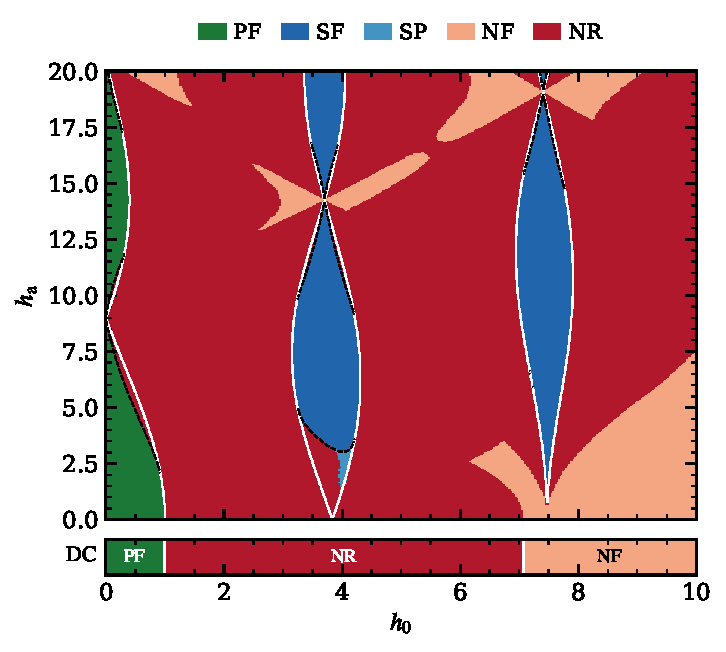
\includegraphics[width=\linewidth]{figuras/phasediagram_L256.pdf}
    \caption{Dynamical phase diagram for an extended domain wall in the large-system limit ($L/L_0 = 256$), showing the five dynamical regimes: pinned flat (PF), synchronized flat (SF), synchronized periodic (SP), non-synchronized flat (NF), and non-synchronized rough (NR), for $\alpha=0.27$ and $\Omega=1$. Continuous white and dashed black curves represent the boundaries of synchrony and linear stability ($\mu=1$) of the corresponding rigid flat wall, respectively. The horizontal strip at the bottom displays the purely DC-driven phases ($h_\mathrm{a}=0$): PF for $0 \le h_0 \le 1$, precessional rough (NR) for $1 < h_0 < h_c$, and precessional flat (NF) for $h_0 \ge h_c$, with $h_c \approx 7.08$. The small-system phase diagram ($L/L_0=8$) is presented separately in Appendix~\ref{ap:finitesizephasediagram}.}
    \label{fig:fases}
\end{figure}
\rec{Figure 5 Label Consistency: In the figure panel and caption, the non-precessional phase is now harmonized to ``PF'' (Pinned Flat) across the figure legend, bottom DC strip, and caption, fully consistent with Table~I and the other two-letter acronyms (SF, SP, NF, NR).}


\begin{table*}[t]
\centering
\begin{tabular}{c|c|c|c}
\hline
Phase 
& $u$ spatial structure 
& $\phi$ synchronization
& DW average precession \\
\hline

PF 
& Flat 
& Pinned 
%($\langle \dot \phi \rangle=0$)
& Absent \\


SF 
& Flat 
& Synchronized 
& Coherent \\

SP 
& Periodic (controlled by Floquet instabilities)
& Synchronized 
& Coherent \\

NF 
& Flat 
& Non-synchronized 
& Coherent \\

NR 
& Rough (Edwards-Wilkinson)
& Non-synchronized 
& Incoherent / chaotic \\
\hline
\end{tabular}
\caption{Characterization of the dynamical phases in terms of the spatial
structure of $u$, synchronization of the domain-wall precession $\phi$
with the external drive, and coherence of the precessional dynamics.
The SF and SP phases are synchronized and exhibit coherent domain-wall
precession, while the NF phase corresponds to coherent but
non-synchronized precession. In the NR phase, the precession becomes
incoherent and chaotic, accompanied by Edwards--Wilkinson roughening of
$u$ in the thermodynamic limit. In the SP phase, the periodic spatial
structure is characterized by a wavelength selected by the narrow band
of linearly unstable modes.}
\label{tab:phases}
\end{table*}

% We are now in position to unveil and discuss the the main result of our paper, the full dynamical phase diagram in the $(h_0,h_a)$ plane for fixed AC frequency.


% Figure~\ref{fig:fases} shows a phase diagram displaying all four possible regimes: synchronized flat (SF), \luzcom{synchronized periodic (SP)}, non-synchronized flat (NF) and \luzcom{non-synchronized rough (NR)}.
% Panel (a) shows the dynamical regimes of a finite-size domain wall, whereas panel (b) presents the corresponding dynamical phase diagram in the thermodynamic limit, where the sharp crossovers sharpen into genuine dynamical phase transitions. These results are generic to systems described by Eq.~\eqref{eq:uphi}. While the quantitative details depend on the value of $\alpha$, different values yield qualitatively similar phase diagrams~\cite{pusiol2026deterministic}. The specific micromagnetic parameters merely set the corresponding field ($H_W$), time ($T_0$), and length ($L_0$) scales. 
% In the following we discuss the different dynamical phases. 
% \color{black}
% \color{blue}

% Overall, the NF and SF phases dominate the behavior of small systems, while for large systems the turbulent NR phase becomes relevant over large regions of the phase diagram. The SP phase on the other hand needs tuning to a reduced region in the $(h_0, h_a)$ diagram.  In the following we focus and discuss the large system thermodynamic behavior Figure~\ref{fig:fases}(b).

% % \alecom{
% % Preguntas:
% % \begin{itemize}
% %     \item Para un $h_0$ dado, puede ser DC corrugado y AC+DC flat, en situacion de sincronia? AC estabilizante?
% %     \item Para un $h_0$ dado, puede ser DC corrugado y AC+DC flat, en situacion de desincronia? AC estabilizante?
% %     \item Para un $h_0, h_a$ dados con sincronia, puede el caso DC+AC ser corrugado y el puro DC flat? AC desestabilizante?
% %     \item Para un $h_0, h_a$ dados con desincronia, puede el caso DC+AC ser corrugado y el puro DC flat? AC estabilizante?
% %     \item Cuan diferentes son los escalones de Shapiro con respecto a los de la rigid DW? Floquet realmente nos da la pista como se modifica?
% %     \item Cual es la naturaleza de la phase NR?
% %     \item Cual es la naturaleza de la phase SP?
% % \end{itemize}
% % }

% We note first that the Arnold tongues of synchrony of the precessional degree of freedom of the extended flexible DW with the external AC drive are close to those of the rigid DW, except in narrow regions close to the Shapiro steps edges and near the occurrence of the SP phase. In those cases, linear stability Floquet analysis better predicts the Arnold tongues that actually occur in the steady-state solution of the full non-linear system. 

% Comparing with the pure DC driven case, the addition of the AC can drive the NR turbulent or the NF pure DC states to synchrony, and depending on its amplitude, to either a SP phase, or into a SF state. It can also drive it to a non-sync AC excited NR state which, as we show below, is in the same universality class of the pure DC turbulent phase. Interestingly, by increasing the AC amplitude $h_a$ we can have a sequence of transitions,  NR $\to$ NF $\to$ NR,  around the crossings of the synchrony boundary lines (this effect could be due to parametric stabilization, analogous to Kapitza's pendulum~\cite{LandauMechanics,kapitza1951}). In summary, the AC drive can be stabilizing or destabilizing on the flat DW structure, and can drive to synchrony or asynchrony. Most of the synchronic cases belong to the SF phase, except for the intriguing SP phase that we discuss in more details below.


% % Except for the SP phase, synchrony appears to flatten the moving DW, leading to the SF phase. Interestingly however, synchrony appears to not be the only mechanism for the AC drive to stabilize the DW, as shown by the butterfly-shaped regions of the NF phase in Fig.~\ref{fig:fases}(b) around the crossings of the synchrony boundary lines (this effect could be due to parametric stabilization, analogous to Kapitza's pendulum~\cite{LandauMechanics,kapitza1951}). The AC drive can also destabilize the flat DW state, even for small systems. 
% % It is clear that the SF regime preserves spatial ordering by flattening the wall, and, as expected, lies within the stability boundaries of the time periodic rigid DW. In the region of instability, there are both \luzcom{SP and NR} regimes. 

% % \subsection{
% % \aleadd{Structure of the 
% % non-flat  phases: SP, NR}
% % }

% We now turn our focus to the nature of the \aleadd{non-flat  phases}, NR and SP.
% % , in order to determine whether the temporal order that remains induces spatial order in a configuration that is not flat. 
% To evaluate the spatial ordering in such a regime, we introduce the structure factor $S_\kappa$, defined as

% \begin{equation}
%     S_\kappa = \left\langle\left|\hat u_\kappa\right|^2\right\rangle_t\, ,
%     \label{eq:factor_estructura}
% \end{equation}
% where the time averaging is done over an integer number of periods of the AC drive, and the global roughness $w^2$, defined in Eq. \eqref{eq:roughnessvst}. 


% Fig.~\ref{fig:estructura} shows the typical behavior found in the transient surface growth regime that converges to the NR phase at long times. The structure factor, in Fig.~\ref{fig:estructura}(a), is approximately described by $S_\kappa \propto \kappa^{-2} F(\kappa l(t))$ with $l(t)\sim t^{1/2}$ a growing correlation length and $F(x)$ a function such that $F(x)\sim x^{2}$ for $x \ll 1$ and $F(x)\sim \mtext{const}$ for $x\gg 1$. The DW rugosity $\langle w^2 \rangle_t$ on the other hand,  in Fig.~\ref{fig:estructura}(a), displays a growth regime characterized by $\langle w^2 \rangle_t  \propto t^{1/2}$. These results are consistent with the Edwards-Wilkinson surface growth universality class \cite{barabasi1995fractal}, which predicts $S(\kappa) \sim \kappa^{-(1+2\zeta)}F(\kappa t^{1/z})$ and $\langle w^2 \rangle_t \propto t^{2\zeta/z}$ with roughness exponent $\zeta=1/2$ and dynamical exponent $z=2$. These results confirm that the NR regime belongs to the 1D Edwards-Wilkinson universality class, as in the DC-only case.


% % dominated at low frequencies by a power law behaviour $S_\kappa \propto \kappa ^{-2}$, as shown in Fig.~\ref{fig:estructura} \textbf{(a)}. Furthermore, analysis of the evolution of the DW rugosity $w^2$ as a  function of time shows that the DW enters a growth regime characterized by $w^2\propto t^{1/2}$, as demonstrated in Fig. \ref{fig:estructura} \textbf(b). These results confirm that the NR regime belongs to the 1D Edwards-Wilkinson universality class, as in the DC-only case.} 

% We now turn our attention to the nature of the non-flat SP phase that exists in reduced regions of the phase diagram but it is found to be thermodynamically stable. 
% Fig.~\ref{fig:sc_cascade} shows snapshots of the DW at times evenly distributed over two periods of the driving field, in the steady-state. The wall expands vertically, oscillates around this position and then collapses and crosses over, inverting peaks and valleys, entering a regime that is periodic in both space and time. The roughness $\langle w^2 \langle_t$ of the SP phase is constant and independent of $L$ in the large size limit, indicating that the average amplitude of the spatial periodicity is constant. We also observe that very small systems become flat in spite of the $\kappa_{\rm peak}$ instability because of the low density of modes. The time period on the other hand is twice the period of the driving field, while the spatial period is determined by the most linearly unstable mode $\kappa ^\ast$, as can be appreciated in Figure \ref{fig:estructuraSCvsL}(b) in the large $L$ size limit. 
% In summary the SP phase is thermodynamically stable, macroscopically flat but periodically corrugated, and oscilatory in time, reminiscent of a ``time crystal''.


% % \luzcom{The stability of the SP phase in the thermodynamic limit is demonstrated in Fig.~\ref{fig:estructuraSCvsL}, where it is shown that both the rugosity $w^2$ and the dominant spatial frequency $\kappa_\text{peak}$ are stable and independent of system size $L$ for large enough systems. Furthermore, the limiting value of $\kappa_\text{peak}$ is given by $\kappa^\ast$.}

% % If the DW becomes chaotic, we expect that after a long time, the structure factor will be dominated by a power law behavior, similar to the purely DC case. If the DW remains ordered instead, its structure factor should be dominated by peaks at some specific wavenumbers with a low background. Figure~\ref{fig:estructura} shows the steady state $S_\kappa$ for a DW of size $10\,000$, both in the SC ($h_0 = 4,\, h_\text{a} =3$) and NC ($h_0=5,\, h_\text{a} = 3$) phases. The low-$\kappa$ behavior of $S_\kappa$ in the NC regime follows a power law with exponent $-2$. Analysis of the evolution of DW rugosity as a function of time shows that the DW enters a growth regime characterized by $w^2\propto t^{1/2}$. These results are consistent with the 1D Edwards-Wilkinson universality class.
% % \color{blue}
% % Figure~\ref{fig:estructuraNCvsL} shows that $\langle w^2 \rangle_t/L$ approaches a constant for large $L$, consistent with a rough self-affine interface such that $\langle w^2 \rangle_t \sim L^{2\zeta}$, with a roughness exponent $\zeta=1/2$.
% % These results show that the NC phase belongs to the Edwards-Wilkinson universality class at large spatiotemporal scales, with a deterministically induced effective temperature, as is the case for the purely DC-driven DW~\cite{pusiol2026deterministic}.  
% % \color{black} 
% % \luzcom{Fig.~\ref{fig:NChistograma} shows the steady-state distribution of heights for a DW in the NC phase ($h_0=5,\ h_a=3$). It is approximately Gaussian, consistent with the 1D Edwards-Wilkinson universality class.}



\begin{figure}[hbtp]
    \centering
    \begin{overpic}[width=\linewidth]{figuras/NC_EW_inset.pdf}
        \put(72, 58){\textbf{(a)}} 
        \put(72, 13){\textbf{(b)}}
    \end{overpic}
    
    \caption{Universal scaling and exponent analysis of the non-synchronized rough (NR) phase ($h_0=5,\, h_\text{a} = 3,\, \Omega=1,\, \alpha=0.27$, for $L/L_0=1000$). (a) Main panel: Structure factor $S_\kappa$ as a function of wavenumber $\kappa$ at different times $t$ during the transient growth regime, with the dashed line indicating the asymptotic power-law decay $S_\kappa\propto\kappa^{-2}$. Curves are color-coded by time $t$ according to the colorbar above. Inset: Scaling collapse onto the universal master curve $S_\kappa t^{-1}$ versus $\kappa t^{1/2}$, demonstrating dynamic scaling consistent with $S(\kappa,t)\sim \kappa^{-(1+2\zeta)}F(\kappa t^{1/z})$ with roughness exponent $\zeta=1/2$ and dynamic exponent $z=2$. (b) Domain-wall roughness $w^2$ as a function of time $t$; the dashed line illustrates the characteristic growth regime $w^2\propto t^{1/2}$. These scaling relations confirm that the NR phase under combined DC+AC driving belongs to the one-dimensional Edwards--Wilkinson universality class.}    
    \label{fig:estructura}
\end{figure}


% % On the contrary, in Fig.~\ref{fig:estructura} we see that the structure factor of the SC phase is essentially zero at most wavenumbers, except for narrow peaks at $\kappa \approx0.84$ and its harmonics. 
% % This demonstrates that the SC phase achieves a stable and ordered spatial configuration. 

% % To show that this order is independent of system size in the thermodynamic limit, we show in Fig.~\ref{fig:estructuraSCvsL} that the wavenumber of the first peak $\kappa_\text{peak}$ and the steady-state rugosity $\left\langle w \right\rangle_t$ reach a constant for large $L$, consistent with long range order of periodicity. The figure also displays the wavenumber corresponding to the maximum Floquet multiplier $\kappa^\ast$, which demonstrates that the periodicity is intrinsically dominated by this single mode. Interestingly, synchronization in this phase inhibits the cascade of mode-mode interactions that lead to the spatiotemporal chaos in the pure DC case~\cite{pusiol2026deterministic}. 
% %\color{blue}
% %To show that this spatial order is independent of system size in the thermodynamic limit in Fig.~\ref{fig:estructuraSCvsL}  we show that the location of the first peak $\kappa_{\rm peak}$ and its normalized magnitude $S(\kappa_{\rm peak})/L$ reach a constant for large $L$, consistent with a long-range order with periodicity $\sim \kappa_{\rm peak}^{-1}$. The figure also display the band of linearly unstable modes, evidencing that the periodicity is mainly controlled intrinsically by these modes. Interestingly, synchronization in this SC phase, inhibits the cascade of mode-mode interactions that leads to the spatiotemporal chaos observed in the pure DC case~\cite{pusiol2026deterministic}.
% %\color{black}

% % Figure~\ref{fig:snaps} shows snapshots of this configuration taken at even intervals over a single period of the DW in the steady state. The wall breathes at a frequency that is half of the driving frequency, while maintaining a structure dominated by a single spatial frequency and its harmonics. These results show that a long-range spatiotemporal order emerges in the SC phase. 


% % \begin{figure}[hbtp]
% %     \centering
% %     %\includegraphics[width=\linewidth]{}
% %     \caption{
% %     \color{blue}
% %     Finite size analysis of the NC, spatiotemporal chaotic rough phase.
% %     \color{red}        (Luz)
% %     \color{black}
% %     }
% %     \label{fig:estructuraNCvsL}
% % \end{figure}



\begin{figure}[hbtp]
    \centering
    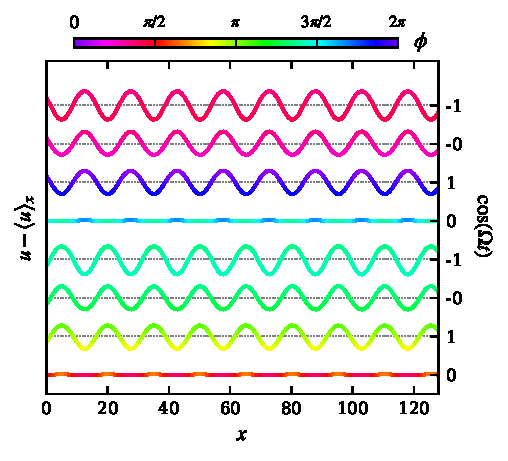
\includegraphics[width=\linewidth]{figuras/sc_cascade.pdf}
    \caption{\luzcom{Propuesta 2 (cascada)\\
    Snapshots of a section of the DW in the steady-state SC regime ($h_0=4, \, h_\text{a}=3,\, \alpha=0.27$ and $\Omega=1$), taken at evenly spaced intervals over a full period of its motion. 
    }}
    \label{fig:sc_cascade}
\end{figure}
\rec{Figure 7 Caption Clean-up: (i) Remove the Spanish draft title ``Propuesta 2 (cascada)''. (ii) Update ``SC regime'' to ``SP phase'' to match Table~I. (iii) Suggested clean caption: ``Spatiotemporal profiles of a section of the domain wall in the steady-state synchronized periodic (SP) phase ($h_0=4,\, h_\text{a}=3,\, \alpha=0.27$, and $\Omega=1$), displayed at evenly spaced intervals over one full driving period $T = 2\pi/\Omega$. The wall undergoes periodic transverse breathing and inversion without developing a turbulent cascade into higher spatial modes.''}

\begin{figure}[hbtp]
    \centering
    \begin{overpic}[width=\linewidth]{figuras/SC_scaling.pdf}
        \put(90, 52){\textbf{(a)}}
        \put(90, 17){\textbf{(b)}}
    \end{overpic}
    \caption{\luzcom{
     Finite size analysis of the SC phase. (a) DW rugosity $\langle w^2 \rangle_t$ and (b) wavenumber of the maximum peak in the structure factor $\kappa_\text{peak}$ as a function of $L/L_0$. The long range spatiotemporal order is dominated by the most linearly unstable mode $\kappa^\ast$ (dotted line) of the synchronized phase. For large enough systems, the roughness converges to a constant value independent of system size. For small sizes, the structure factor is dominated by the lowest available mode $2\pi/(L/L_0)$ (dashed line) and the DW is flat due to the lack of modes in the narrow instability band.
     }}
    \label{fig:estructuraSCvsL}
\end{figure}
\rec{Figure 8 Caption Harmonization: Change ``SC phase'' $\to$ ``SP phase''. Note that in panel (a), roughness saturates to a size-independent constant $\langle w^2\rangle_t \approx 0.05$ as $L \to \infty$, demonstrating genuine long-range periodic order in sharp contrast to the self-affine divergence $\langle w^2\rangle_t \propto L$ characteristic of the rough NR phase.}

% % \begin{table*}[t]
% % \centering
% % \begin{tabular}{lll}
% % \hline
% % Phase & Synchronization & Spatial order \\
% % \hline
% % SP & Frequency-locked to the external drive
% %    & Periodic corrugation (selected unstable wavelength) \\
% % SF & Frequency-locked to the external drive
% %    & Flat \\
% % NR & No frequency locking; chaotic/turbulent dynamics
% %    & Rough (EW) \\
% % NF & No frequency locking; coherent drift
% %    & Flat \\
% % \hline
% % \end{tabular}
% % \caption{
% % \color{blue}
% % Summary of the dynamical phases. The SC phase exhibits a periodically corrugated profile whose characteristic wavelength is selected by the narrow band of linearly unstable modes. The NC phase is corrugated but lacks spatial long-range order, displaying Edwards--Wilkinson (EW) roughening in the thermodynamic limit.
% % \color{black}
% % }
% % \label{tab:phases}
% % \end{table*}


% % \alecom{Falta mucha discusion:
% % \begin{itemize}
% %     \item NC: es turbulenta siempre? \luzcom{turbulenta sería temporalmente?}\underline{\textbf{Propuesta (Luz) #1}}: agarrar una NC y dibujar el ruido de baja frecuencia de la velocidad precesional y la otra tambien.
% %     \luzcom{de la NC me falta hacer la figura del scaling con $L$, está en camino
% %     }
% %     % y $\langle w^2 \rangle/L$
% %     % vs $L$ de $L$ chico hasta $L$ grande, termodinamico. También se podría mostrar $S(\kappa \approx 0)/L^2$ para $h_0=5$ y $h_a=3$ para distintos $L$, ya que $S \sim L^2$ y deberian colapsar las curvas ahi.
    
% %     \item  \sout{SC: La periodicidad espacial de esta determinada por los modos linealmente inestables?\luzcom{Sí!} En la Fig4a parece que $0.75<\kappa<0.95$ pasa algo. \underline{\textbf{Propuesta (Luz) #2}}: Agarrar una SC de ejemplo y dibujar ambos, $S(\kappa_{peak})$ (debidamente normalizado por una potencia de $L$) o  $\langle w^2 \rangle$ vs $L$ y $k_{peak}$ vs $L$. Y ahi mismo comparar con el $\kappa^*$ donde $\mu_{\kappa^*}$ es maximo o la banda donde $\mu > 1$. Mostramos que mas o menos ahi satura a $L$ grande.} 
    
% %     \item SC: hay que argumentar porque siendo que hay modos inestables estos no dan lugar a cascadas y al caos... posiblemente la sincronia mate cascada.
% %     \item 
% %     Falta discutir de que depende el periodo espacial de la SC. Pareciera venir de la estabilidad lineal, podemos chequearlo? que tiene el 0.84 de especial por ejemplo? 
% %     En la Fig4a parece que $0.75<\kappa<0.95$ pasa algo. Pero va a quedar claro con la figura de la propuesta 2.
% %     \luzcom{si entiendo bien esto ya está}
% %     \item NC: Falta mostrar que en la NC la distribucion de alturas de la interface es gausiana, asi podemos descartar KPZ que tambien tiene $\zeta=1/2$. Lo hicimos sin AC, pero no sabemos que pasa con AC. \underline{\textbf{Propuesta (Luz) 3}}: Calcular la PDF/histograma de $u$ a tiempos largos en un ejemplo de NC. Puede ir a parar al apendice.
% %     \item NC: Mencionar algo de la $T_{\rm eff}$, de que depende?. $S(\kappa)\sim T_{\rm eff}\kappa^{-2}$. Seguramente de los $\mu_\kappa$...


% % \end{itemize}
% % }





% Table~\ref{tab:phases} summarizes the main properties and the spatiotemporal order of each dynamical phase in the phase diagram of Figure \ref{fig:fases}. 





%%%%%%%%%%%%%%%%%%%%%%%
\section{Dynamical Phases}\label{sec:dynamicalphases}

% We are now in a position to discuss the main result of this work: the full dynamical phase diagram in the $(h_0,h_a)$ plane at fixed AC frequency. Figure~\ref{fig:fases} shows \aleadd{five} distinct dynamical regimes:
% pinned flat (PF), 
% synchronized flat (SF), synchronized periodic (SP), non-synchronized flat (NF), and non-synchronized rough (NR). 
% The phase diagram corresponds to $L/L_0=1000$, for which size effects are already negligible.
% Finite size effects become however visible for much smaller systems (see appendix \ref{ap:finitesizephasediagram}). 
% We can thus consider that the dynamical regimes of Figure~\ref{fig:fases} represent the $L\to\infty$ dynamical phases.
% Synchronization is identified by $\sigma<0.01$. The continuous and dotted gray lines indicate, respectively, the synchronization boundaries and the linear-stability boundaries of the corresponding synchronized flat rigid-wall solutions.
% Note that by construction, the interior of the dotted line is strictly contained in the interior of the continuous line. The complement thus corresponds to unstable flat DWs.
% \fabriq{Aquí cuando hablamos de los límites de estabilidad lineal, podríamos aclarar que la línea punteada marca el límite inferior (onset) de la región de estabilidad y lo que queda por debajo es inestable.}


We are now in a position to discuss the main result of this work: the full dynamical phase diagram in the $(h_0,h_a)$ plane at fixed AC frequency. Figure~\ref{fig:fases} shows five distinct dynamical regimes: pinned flat (PF), synchronized flat (SF), synchronized periodic (SP), non-synchronized flat (NF), and non-synchronized rough (NR). The phase diagram corresponds to $L/L_0=1000$, for which finite-size effects are negligible on the scale considered. Finite-size effects become visible for substantially smaller systems (see Appendix~\ref{ap:finitesizephasediagram}), so we use the $L/L_0=1000$ results as representative of the $L\to\infty$ dynamical phase diagram. Synchronization is identified by $\sigma<0.01$. The continuous and dotted gray lines indicate, respectively, the synchronization boundaries and the linear-stability boundaries of the corresponding synchronized flat rigid-wall solutions. These boundaries provide a reference for the long-time dynamics of the full nonlinear extended-wall equations: the continuous lines delimit the parameter regions where the corresponding rigid-wall solutions are synchronized, while the dotted lines indicate where these synchronized flat solutions become spatially unstable.
\rec{System Size Accuracy in Text: Change ``$L/L_0=1000$'' to ``$L/L_0=256$'' (in both sentences) to match Figure~\ref{fig:fases} and its caption where the simulated large system is explicitly $L/L_0=256$.}


In the PF phase, $\langle\dot{\phi}\rangle=0$, so the DW does not exhibit average internal precession, although its mean position $\langle u\rangle$ can still evolve in time. The effective Walker breakdown field in presence of AC drive follows $h_W \approx |J_0(\alpha h_a/\Omega)|$, as predicted by the equality in Eq.\eqref{eq:walkerwithAC} for the particular $n=0$ case. The remaining four regimes combine temporal synchronization with distinct spatial structures. The SF and SP phases are synchronized, whereas NF and NR are non-synchronized. Spatially, SF and NF remain essentially flat, while SP develops a periodic corrugation and NR exhibits roughening. 
The SP regime occupies a comparatively narrow regions, for relatively low values of $h_a$, at the bottom of the synchronization regions. 
\rec{Typo: Change ``occupies a comparatively narrow regions'' $\to$ ``occupies a comparatively narrow region''.}
% In the following, we focus on the large-system behavior and characterize the spatial and temporal properties of the different regimes.

The synchronization regions of the extended domain wall remain close to those obtained from the rigid-wall dynamics (delimited by the continuous lines) over most of the phase diagram. These lines are described by Eqs.\eqref{eq:walkerwithAC} and \eqref{eq:width_steps}. 
Deviations due to the flexural modes of the extended DW are most pronounced near the edges of the synchronization steps and in the region where the SP state develops. In these regions, the Floquet stability analysis of the synchronized rigid-wall solution provides a direct indication of the onset of spatial instabilities (indicated by the dotted lines). In Fig. \ref{fig:fases} we also observe that the dotted lines provide an approximation for the onset of instabilities inside the synchronized phase of the rigid DW.
Thus, synchronization and spatial stability are related but distinct properties of the driven wall. 
\rec{Clarification of Dotted Stability Boundary (Addressing Fabricio's note): Clarify in the text that the dotted line marks the lower onset of linear stability for the synchronized flat state: the region below this dotted line is linearly unstable to flexural corrugations, explaining why the SP phase appears precisely in the unstable sub-tongue where synchrony holds but flat walls destabilize.}

The AC drive can qualitatively modify the dynamics observed under pure DC driving. It can suppress roughening and stabilize a synchronized flat state, or it can synchronize a spatially unstable state, leading to the SP regime. Conversely, non-synchronized flat states can also occur under AC driving. The resulting phase diagram therefore reflects the interplay between temporal synchronization and spatial stability rather than a single synchronization transition.
Since the flat phases indistinguishable from the rigid-wall solutions, in the following we solely characterize the non-flat phases.
\rec{Grammar Typo: Change ``Since the flat phases indistinguishable'' $\to$ ``Since the flat phases are indistinguishable''.}


We first characterize the NR regime. To quantify its spatial structure, we analyze the roughening process and consider the \textit{time-dependent} structure factor starting from an initially perturbed flat DW
\begin{equation}
    S_\kappa = \left\langle\left|\hat u_\kappa(t)\right|^2\right\rangle ,
    \label{eq:factor_estructura}
\end{equation}
and the \textit{time-dependent} global roughness 
\begin{equation}
w^2 =
\left\langle u^2(t)\right\rangle_x
-\left\langle u(t)\right\rangle_x^2
.
\label{eq:roughness}
\end{equation} 
where the averages are done over random realizations of the perturbed initial DW. 


During the transient growth regime that nucleates the NR phase, 
shown in Fig.~\ref{fig:estructura},
the structure factor follows the scaling form
\begin{equation}
S_\kappa \propto \kappa^{-2}F(\kappa \, l(t)),
\end{equation}
with a growing length-scale $l(t)\sim t^{1/2}$, while $F(x)\sim x^2$ for small $x$ and approaches a constant for large $x$.
As shown in the inset of Fig.~\ref{fig:estructura}(a), the rescaled data $S_\kappa t^{-1}$ collapse onto a single universal curve when plotted against $\kappa t^{1/2}$.
Correspondingly, the roughness grows as
\begin{equation}
w^2 \propto t^{1/2}.
\end{equation}
These scaling properties are consistent with the one-dimensional Edwards--Wilkinson universality class, where $w^2 \sim t^{2\zeta/z}$ and $S(q)\sim q^{-(1+2\zeta)}F(q t^{1/z})$, with a roughness exponent $\zeta=1/2$ and dynamic exponent $z=2$. The NR phase under DC+AC drive is thus in the same the universality class as in the purely DC-driven case \cite{pusiol2026deterministic}.
\rec{NR Universality \& Effective Temperature (Addressing Ale's note): (i) Typo: ``same the universality class'' $\to$ ``same universality class''. (ii) Add: ``Furthermore, the steady-state structure factor exhibits an asymptotic $S(\kappa) \approx T_{\rm eff} / \kappa^2$ divergence, reflecting a deterministically induced effective temperature $T_{\rm eff}$ originating from chaotic Bloch line nucleation and collisions. The height distribution $P(u)$ is Gaussian with vanishing skewness, ruling out Kardar--Parisi--Zhang (KPZ) universality and confirming linear Edwards--Wilkinson scaling under AC driving.''}

We next turn to the SP regime. Figure~\ref{fig:sc_cascade} shows representative configurations over two periods of the AC drive. The wall develops a periodic corrugation whose amplitude oscillates in time, while the spatial profile recurs periodically. The roughness approaches a finite value as the system size increases, and the dominant wave number remains finite, indicating that the corrugation is not a finite-size artifact. 
\rec{Mechanism of Cascade Arrest in the SP Phase (Addressing Ale's note): Explain why unstable modes do not trigger spatiotemporal chaos: ``Remarkably, despite possessing a finite band of linearly unstable modes, the SP phase does not degenerate into spatiotemporal chaos. Strong temporal phase-locking to the AC drive rigidly pins the phase of the dominant mode $\kappa^*$. This phase coherence arrests the multi-wave resonant interactions that otherwise drive an energy cascade toward higher and lower modes in the purely DC regime~\cite{pusiol2026deterministic}, trapping the system in a stable, periodically corrugated limit cycle.''} 

The spatial periodicity of the SP phase is directly related to the Floquet instability of the synchronized flat state. In the unstable region, a finite band of wave numbers has Floquet multipliers larger than unity, with a maximum growth rate at a characteristic wave number $\kappa^*$. The nonlinear SP state is dominated by a wave number $\kappa_{\rm peak}$ that approaches a finite value with increasing system size and is consistent with the Floquet-selected $\kappa^*$ (indicated by the dashed horizontal line). Figure~\ref{fig:estructuraSCvsL} shows that both the roughness and $\kappa_{\rm peak}$ converge as $L$ increases. For sufficiently small systems, the allowed wave numbers may not sample the unstable band adequately; in that case the wall can remain effectively flat even when the corresponding continuum system is spatially unstable.

The finite-size analysis therefore demonstrates that the periodic corrugation in the SP regime has an intrinsic spatial scale selected by the linear instability of the synchronized state. In the large-system limit, the SP phase exhibits long-range spatial periodic order together with temporal synchronization.

The main properties of the five dynamical phases are summarized in Table~\ref{tab:phases}.
%%%%%%%%%%%%%%%%%%%%%%%















\section{Conclusions}\label{sec:conclusions}
We investigated synchronization in extended domain walls driven by combined DC and AC magnetic fields and its relation to spatial order. We showed that synchronization can occur even in very large systems exhibiting spatiotemporal chaos in the purely DC-driven regime. Synchronization is generally accompanied by a suppression of this chaotic dynamics and, in most cases, by a flattening of the domain wall. However, synchronized regimes with a periodically corrugated spatial structure also exist. In this regime, the corrugation is dominated by a finite band of linearly unstable modes with a well-defined maximum growth rate, linking the spatial structure of the nonlinear state to the Floquet instability of the synchronized flat state. The resulting dynamical phase diagram, shown in Figure~\ref{fig:fases}, summarizes these different regimes.

The AC field amplitudes required to drive a chaotic domain wall into the SP phase are of the order of the Walker field. For a thin Co/Pt multilayer, the minimum AC amplitude required is of order $10$ mT, with frequencies on the order of $100$ MHz. These conditions are experimentally accessible (see Appendix~\ref{ap:exp_cond} for the correspondence between the model parameters and physical units). The finite-size effects identified in this work may also be relevant for experimentally accessible micrometer-scale systems.

The framework developed here neglects disorder and thermal fluctuations \cite{ferre2013,ferrero2021creep}, which may affect the experimental observation of the predicted dynamical regimes. Nevertheless, the present theory provides a basis for extending the analysis to more realistic domain-wall models that incorporate these effects. The framework can also be generalized to higher-dimensional geometries and to electrical current drives, providing directions for future studies.

Beyond these extensions, our results demonstrate that a spatially extended nonlinear system exhibiting deterministic spatiotemporal chaos can synchronize to an external periodic drive. We further show that synchronization can suppress the chaotic dynamics while preserving spatial structure, leading either to a synchronized flat state or to a synchronized periodically corrugated state with long-range spatiotemporal periodic order. This coexistence of temporal synchronization and spatial instability provides a distinctive dynamical regime of driven precessing domain walls.
\rec{Conclusions Enhancement --- Spintronic Outlook: Add an outlook paragraph on spin-orbit torques and device applications: ``In addition to magnetic field driving, equivalent effective driving forces can be exerted through spin-orbit torques (SOT) in heavy-metal/ferromagnet bilayers (such as Pt/Co/AlOx). Radio-frequency AC currents in the gigahertz regime can deliver effective field amplitudes of tens of milliteslas, providing a versatile on-chip platform to observe these synchronization-induced transitions. Technologically, the ability to switch deterministically between flat (high mobility) and corrugated (low mobility) states under AC gating offers a promising mechanism for low-power spintronic microwave detectors, frequency filters, and physical reservoir computing.''}

\begin{acknowledgments}
We thank T. Giamarchi for discussions. Simulations used the Gerencia de Física  HPC cluster at CAB-CNEA (SNCAD, Argentina).
\end{acknowledgments}


\appendix

\section{Experimental conditions}
\label{ap:exp_cond}

We work out the conversion of our nondimensional model into physical units for the case of a standard Co/Pt multilayer, with parameters~\cite{skaugen2019} $\alpha=0.27$, $A_\text{ex}=1.4 \times 10^{-11}$~J/m, $M_\text{s}=9.1\times 10^5$~A/m, $K_\text{u}=8.4\times 10 ^5$~J/m$^3$ and $N_\text{n}=0.016$.

The length scales for this material are $\Delta\approx6.6$~nm and $L_0\approx8.77\Delta\approx58.0$~nm. This means that the values of $L/L_0$ of 7, 1000, and $10\,000$ in units of $L_0$ used throughout our work correspond to DWs of lengths 406~nm, $58.0$~$\mu$m, and $580$~$\mu$m, respectively. The limiting thermodynamic behavior begins to occur for lengths of order $100\, L_0\approx5.8$~$\mu$m.
\rec{Physical Length Scales Update: Update the representative values of $L/L_0$ from obsolete values ($L/L_0=7, 1000, 10000$) to the actual simulation sizes used in the paper: $L/L_0=8$ ($\approx 464$~nm), $L/L_0=256$ ($\approx 14.8$~$\mu$m), and $L/L_0=1024$ ($\approx 59.4$~$\mu$m). Note that $L/L_0=1000$ corresponds to $58.0$~$\mu$m, while the finite-size scaling in Fig.~\ref{fig:estructuraSCvsL} extends up to $L/L_0 \approx 2.6\times 10^5 \approx 15$~mm.}

The time unit in this system is $T_0 \approx0.33$~ns, which corresponds to a frequency unit of $3.03$~GHz. The angular frequency $\Omega=1$ used in this work corresponds to a real frequency of 480~MHz. The wavelength corresponding to this frequency is $0.6$~m, many orders of magnitude above both length scales of the system. 

The Walker breakdown field is $H_\text{W}\approx2.48$~mT. As a specific example, to drive the system in the SF regime at $H_0=4H_\text{W}\approx10$~mT, with a frequency of $\Omega=1$ (480~MHz), the AC field amplitude should be at least $H_\text{a}\approx3.5H_\text{W}\approx9$~mT.

\section{Numerical methods}
\label{ap:num_met}

All systems of ordinary differential equations (ODEs) were solved using a fourth-order Runge-Kutta method \cite{press2007numerical}. This includes the system of two coupled, non-autonomous nonlinear ODEs for the Walker model of rigid DWs, Eqs.~\eqref{eq:walker_tau1} and~\eqref{eq:walker_tau2}, and the linear system of ODEs, Eq.~\eqref{eq:linearized_mode}, used to find the Floquet multipliers of the synchronized rigid wall solution in the extended DW model in Section \ref{sec:flat_sync}.

The partial differential equations (PDEs) for the full $u$--$\phi$ model (Eqs. \eqref{eq:uphi}) were solved using a pseudo-spectral Crank-Nicolson scheme, following the method outlined by Pusiol et al.~\cite{pusiol2026deterministic}. To do this, we first note that by defining the complex variable~\cite{skaugen2022}
\begin{equation}
    z(x,t)=u(x,t)-i\phi(x,t)\, ,
    \label{eq:z_def}
\end{equation}
the $u$--$\phi$ model is equivalent to the single complex PDE
\begin{equation}
    \dot z = \frac{\alpha-i}{2}[\alpha h(t) + i \sin\left(2\operatorname{Im}(z)\right)+z'']\, .
    \label{eq:z_eq}
\end{equation}

Now we separate the right-hand side of Eq.~\eqref{eq:z_eq} into a linear and a nonlinear part:
\begin{equation}
\begin{split}
    \mathcal L(z) &= \frac{\alpha-i}{2}z'' \, ,\\
    \mathcal{N}(z)&=\frac{\alpha-i}{2}[\alpha h(t)+i\sin\left(2\operatorname{Im}(z)\right)]\ .
\end{split}
    \label{eq:lin_nonlin}
\end{equation}

The linear term is stepped according to the Crank--Nicolson method, and the nonlinear term is stepped with an explicit Euler step:

\begin{equation}
\frac{z^{n+1}-z^{n}}{\delta t}=\frac 1 2 \mathcal L(z^{n+1}+z^{n})+\mathcal N(z^n)\, .
    \label{eq:stepping}
\end{equation}

By transforming to Fourier space, $\hat {\mathcal {L}}_k=-\frac{\alpha-i}{2}k^2$, and we can derive an explicit formula for the evolution of the $k$-th Fourier mode:

\begin{equation}
    z^{n+1}_k=\frac{\left(1+\frac{\delta t}{2}\hat{\mathcal L}_k\right)z_k^n+\delta t \widehat{\mathcal N(z^n)}_k}{\left( 1-\frac{\delta t} {2} \hat {\mathcal L}_k \right)} \, .
\end{equation}

At each step, the nonlinear term is calculated in real space and then Fourier transformed. This requires tracking $z$ in both real and Fourier space.


We implemented this method in C++ and CUDA C++, developing an implementation-agnostic interface that allows us to run identical simulations on either a CPU or a GPU, as needed. The GPU implementation outperformed the CPU for system sizes requiring about $1\,000$ samples of $z$, and was essential in order to study system sizes bigger than $L/L_0=1000$. 

We chose the spatial resolution such that macroscopic properties are stable and the smallest features are resolved. Then, we picked a time resolution $dt$ small enough that results are independent of small variations. 

% \alecom{
% Luz: Aqui falta hablar de:
% \begin{itemize}
% \item tamaño de paso temporal,
% \item estudio de convergencia,
% \item tiempo de integración,
% \item sensibilidad a discretización espacial.
% \end{itemize}}
\rec{Appendix B Numerical Details (Addressing Ale's note): Provide concrete numerical parameters to complete this section: ``In our simulations, we used a spatial discretization step $\Delta x = 0.5\,L_0$ (corresponding to $\approx 29$~nm in physical units, well below the characteristic Bloch line width), discretizing a system of size $L/L_0=1000$ into $N = 2048$ grid points (or $N = 16384$ for $L/L_0=10\,000$). The integration time step was fixed to $\delta t = 0.005\,T_0 \approx 1.65$~ps (corresponding to $\approx 1256$ steps per drive cycle at $\Omega=1$), which ensures numerical stability and prevents aliasing in the explicit nonlinear step. Total integration times ranged from $t_{\rm max} = 2000\,T_0$ to $5000\,T_0$ ($\approx 0.66$--$1.65\,\mu$s), discarding initial transients of at least $1000\,T_0$ before computing time averages. Numerical convergence was verified by halving the time step ($\delta t = 0.0025\,T_0$) and doubling the spatial resolution ($\Delta x = 0.25\,L_0$), confirming that steady-state velocities, roughness, and structure factor peak locations remain invariant to within numerical precision.''}

The source code for the simulator is freely available in Ref.~\onlinecite{github_luz}. 

\section{Finite Size Effects}
\label{ap:finitesizephasediagram}
\begin{figure}[hbtp]
    \centering
    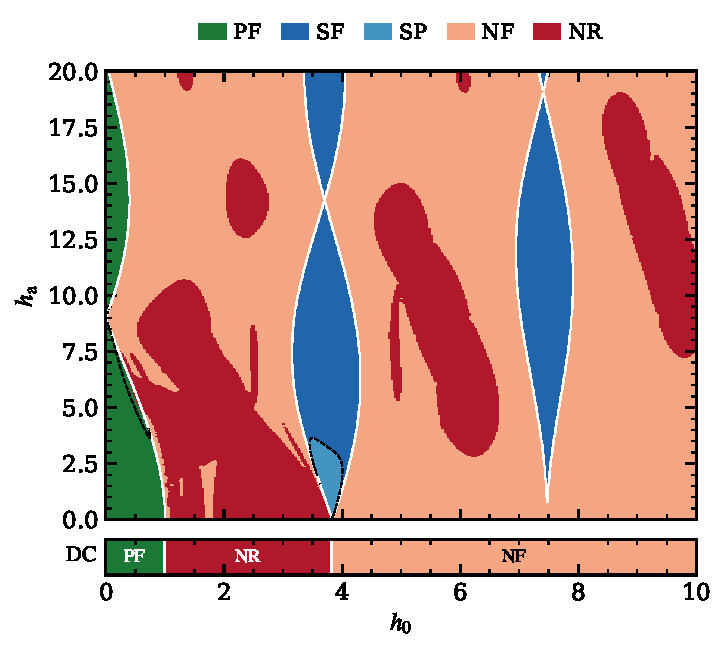
\includegraphics[width=\linewidth]{figuras/phasediagram_L8.pdf}
    \caption{Dynamical phase diagram for a small extended domain wall of size $L/L_0 = 8$, driven by combined DC and AC magnetic fields with $\alpha=0.27$ and $\Omega=1$. The five dynamical regimes are: pinned flat (PF), synchronized flat (SF), synchronized periodic (SP), non-synchronized flat (NF), and non-synchronized rough (NR). Continuous white and dashed black curves indicate the rigid-wall synchrony and linear-stability boundaries, respectively. The horizontal strip at the bottom corresponds to purely DC driving ($h_\mathrm{a} = 0$), showing the non-precessional regime (PF, $0 \le h_0 \le 1$), the precessional rough regime (NR, $1 < h_0 < h_c$), and the precessional flat regime (NF, $h_0 \ge h_c$), where $h_c \approx 3.8$ for $L/L_0=8$ due to the discrete mode spectrum.}
    \label{fig:phasediagram_smallL}
\end{figure}


In Figure~\ref{fig:phasediagram_smallL}, we show the dynamical phase diagram for a relatively small system, $L/L_0=8$. The differences with the large-system phase diagram (Figure~\ref{fig:fases}) highlight the pronounced role of finite-size effects. In particular, for the small system, the discrete set of allowed spatial modes $\kappa_n = 2\pi n / (L/L_0) \approx 0.785 n$ limits the availability of modes that can fall within the linear instability band of the precessing DW. Under purely DC driving ($h_\mathrm{a} = 0$), shown in the horizontal strip below the diagram, the first flexural mode $\kappa_1 \approx 0.785$ is only unstable within a restricted window $1 < h_0 < h_c$, where $h_c \approx 3.8$. For $h_0 > h_c$, all available discrete modes become linearly stable, so the domain wall precesses as a flat interface (NF phase), in sharp contrast with the thermodynamic limit ($L\to\infty$), where the dense spectrum of long-wavelength modes sustains the chaotic NR regime up to $h_c \approx 7$. Similarly, under AC driving, the SF and NF phases dominate a broader region of the phase diagram in the small system, while the chaotic NR regime is significantly reduced compared to large systems. 




\section{Second-order perturbation theory for rigid DW synchrony}
\label{ap:segundo_orden}

We can continue the expansion of Eq.~\eqref{eq:expansion2} to second order in $\epsilon$. To do this we expand $\epsilon\sin(\psi_1) \approx \epsilon \sin\left(\psi^{(0)}\right) + \epsilon^2 \psi^{(1)} \cos\left(\psi^{(0)}\right)$, substitute into Eq.~\eqref{eq:walker_pert} and collect the terms of order $\epsilon^2$. We obtain:
%
\begin{equation}
\dot{\psi}_1^{(2)} = \tilde h_0^{(2)} - \psi^{(1)} \cos\left(\psi^{(0)}\right).
    \label{eq:dot_psi_2}    
\end{equation}

To find $\psi^{(1)}$, we integrate Eq.~\eqref{eq:dot_psi_1} using the Jacobi-Anger expansion for $\sin\left(\psi^{(0)}\right)$ and substituting $\tilde h_0^{(1)}$ from Eq.~\eqref{eq:firstorder}. This yields:
%
\begin{equation}
    \psi^{(1)}(\tau) = \sum_{m \neq -n} \frac{J_m(\tilde h_\text{a})}{n+m} \cos[(n+m)\tau + \psi_\text{c}].
\end{equation}

In order for the second-order solution to remain bounded and $2\pi$-periodic, we require again that the time average of Eq.~\eqref{eq:dot_psi_2} vanishes: $\tilde h_0^{(2)} = \left\langle \psi^{(1)} \cos\left(\psi^{(0)}\right) \right\rangle_\tau$. To compute this average, we expand $\cos\left(\psi^{(0)}\right)$ analogously to the sine term:
%
\begin{equation}
    \cos\left(\psi^{(0)}\right) = \sum_{k=-\infty}^{\infty} J_k(\tilde h_\text{a}) \cos[(n+k)\tau + \psi_\text{c}].
\end{equation}

In the product $\psi^{(1)} \cos\left(\psi^{(0)}\right)$, the time average of terms of the form $\langle \cos(p\tau+\psi_\text{c}) \cos(q\tau+\psi_\text{c}) \rangle_\tau$ is non-zero only when $p=\pm q$. Filtering these resonant terms leads to two contributions to the second-order correction:
%
\begin{equation}
    \tilde h_0^{(2)} = A + B \cos(2\psi_\text{c}),
    \label{eq:secondorder_h0}
\end{equation}
%
where, using the identity $J_{-v}(x) = (-1)^v J_v(x)$, we define the summation constants $A$ and $B$ as:
%
\begin{align}
    A &= \frac{1}{2}\sum_{m\neq -n} \frac{J_m^2(\tilde h_\text{a})}{n+m}, \\
    B &= \frac{1}{2}\sum_{m\neq -n} (-1)^m \frac{J_m(\tilde h_\text{a})J_{2n+m}(\tilde h_\text{a})}{n+m}.
\end{align}

However, shifting the index in our expression for B to $r=n+m$, we can rewrite to obtain:
%
\begin{equation}
    B=\frac{1}{2}\sum_{r\neq 0} \frac{J_{r-n}(\tilde h_\text{a})J_{-r-n}(\tilde h_\text{a})}{r}=0,
\end{equation}
%
since the sum terms are odd in $r$. This simplifies Eq.~\eqref{eq:secondorder_h0} to $\tilde{h}_0^{(2)}=A$. Also note that $A=0$ if $n=0$, for similar reasons. The second order corrections vanish in the zeroth synchrony step.

Substituting in Eq.~\eqref{eq:secondorder_h0}, the DC field in the synchrony condition becomes:
%
\begin{equation}
    \tilde h_0 \approx n + \epsilon^2A + \epsilon(-1)^n J_n(\tilde h_\text{a})\sin(\psi_c),
\end{equation}
%
or, in the original physical variables,
%
\begin{equation}
    h_0 \approx \frac{n\Omega}{\alpha} + \frac{\alpha}{\Omega}A + (-1)^n J_n(\frac{\alpha}{\Omega} h_\text{a})\sin(\psi_c).
    \label{eq:h0_2order}
\end{equation}
%
This is the same as the first-order case, but with a rigid, field-dependent offset in the center of the synchronization step $\frac{\alpha}{\Omega}A$. Consequently, the only second-order effect is a rigid shift in the synchronization steps, depending only on $\alpha h_\text {a}/\Omega$, while maintaining their widths.

In the limit $h_\text{a}=0$, the only term contributing to $A$ is the one proportional to $J_0$. For $n\neq0$, $A=\frac{1}{2n}$: the shift is towards higher absolute DC fields and decreases with the absolute value of the step index. In the limit of $h_\text{a}\to\infty$, $A\to 0$ due to the decay of the Bessel functions, implying that the second order corrections are most significant for small AC fields.

Figure \ref{fig:ej_walker} compares first and second order approximations for the Shapiro steps location.



% 

\section{\fabriq{Dejo esto para discutir: Diagonalization of the background mode equation}}
\label{app:diagonalization}

The linearized mode equation, Eq.~\eqref{eq:linearized_mode}, reads
%
\begin{equation}
    \partial_\tau \boldsymbol{\eta}_\kappa = \frac{1}{2\Omega}\mathcal{M}_\kappa(\tau)\,\boldsymbol{\eta}_\kappa,
    \label{eq:app_mode_eq}
\end{equation}
%
with $\mathcal{M}_\kappa(\tau) = A_\kappa + \cos\psi_1(\tau)\,B$ and
%
\begin{equation}
    A_\kappa = -\kappa^2\begin{pmatrix}\alpha & -1\\ 1 & \alpha\end{pmatrix}, \quad
    B = 2\begin{pmatrix}0 & 1\\ 0 & -\alpha\end{pmatrix}.
    \label{eq:app_A_B}
\end{equation}
%
$A_\kappa$ has eigenvalues $\Lambda_\pm = \kappa^2(-\alpha\pm i)$, eigenvectors $e_+=(1,i)^T$, $e_-=(1,-i)^T$. With $S=(e_+|e_-)$, $\boldsymbol{\eta}_\kappa = S\mathbf{w}$, Eq.~\eqref{eq:app_mode_eq} becomes
%
\begin{equation}
    \partial_\tau \mathbf{w} = \frac{1}{2\Omega}\big[\Lambda + \cos\psi_1(\tau)\,\tilde B\big]\mathbf{w},
    \label{eq:app_w_frame}
\end{equation}
%
with $\Lambda \equiv \mathrm{diag}(\Lambda_+,\Lambda_-)$ and $\tilde B \equiv S^{-1}BS$,
%
\begin{equation}
    \tilde B = \begin{pmatrix} i-\alpha & \alpha-i\\ \alpha+i & -(i+\alpha)\end{pmatrix}.
    \label{eq:app_Btilde}
\end{equation}

\subsection{Fourier content of the periodic background}
\label{app:fourier}

For a solution locked at rotation number $n$, $\psi_1(\tau)\approx n\tau+\psi_\text{c}+x\sin\tau$, $x\equiv\alpha h_\text{a}/\Omega$, so $\cos\psi_1(\tau)$ is $2\pi$-periodic and
%
\begin{equation}
    \cos\psi_1(\tau) = \sum_{m=-\infty}^{\infty} c_m\, e^{im\tau}.
    \label{eq:app_cos_fourier}
\end{equation}
%
Using the Jacobi--Anger identity as in Eq.~\eqref{eq:avg_walker},
%
\begin{equation}
    c_m = \tfrac12\Big[J_{m-n}(x)\,e^{i\psi_\text{c}} + J_{-m-n}(x)\,e^{-i\psi_\text{c}}\Big],
    \label{eq:app_cm}
\end{equation}
%
with $c_{-m}=c_m^{*}$. At $m=0$, using the locking condition $\epsilon \equiv h_0-n\Omega/\alpha=(-1)^nJ_n(x)\sin\psi_\text{c}$ and the stable branch $(-1)^nJ_n(x)\cos\psi_\text{c}>0$,
%
\begin{equation}
    c_0 = \sqrt{J_n(x)^2-\epsilon^2}\,,
    \label{eq:app_c0}
\end{equation}
%
real, non-negative, and vanishing at the step edges.

\subsection{Single-resonance (two-level) reduction}
\label{app:two_level}

In the interaction picture, $\hat{\mathbf{w}}\equiv e^{-\Lambda\tau/2\Omega}\mathbf{w}$, Eq.~\eqref{eq:app_w_frame} becomes
%
\begin{equation}
    \partial_\tau\hat{\mathbf{w}} = \frac{\cos\psi_1(\tau)}{2\Omega}
    \begin{pmatrix}
    \tilde B_{11} & \tilde B_{12}\,e^{-i\kappa^2\tau/\Omega}\\
    \tilde B_{21}\,e^{i\kappa^2\tau/\Omega} & \tilde B_{22}
    \end{pmatrix}\hat{\mathbf{w}}.
    \label{eq:app_interaction_picture}
\end{equation}
%
Keeping only the term stationary near $\kappa^2\approx m\Omega$ ($c_0$ on the diagonal, $c_m$ off-diagonal) and removing the residual phase via $\hat w_1=e^{-i\delta\tau/2}u_1$, $\hat w_2=e^{i\delta\tau/2}u_2$, $\delta\equiv\kappa^2/\Omega-m$, gives an autonomous $2\times2$ problem with eigenvalues
%
\begin{align}
    \lambda_\pm &= -\frac{\alpha c_0}{2\Omega} \nonumber\\
    &\quad\pm \frac{1}{2\Omega}\sqrt{(1+\alpha^2)|c_m|^2-(c_0+\delta\Omega)^2}.
    \label{eq:app_two_level_eigs}
\end{align}
%
This treats each resonance $m$ as isolated. Combining several by taking the union of their windows overestimates the true unstable region, since it discards coupling between near-degenerate channels -- removed next.

\subsection{General multi-harmonic secular expansion}
\label{app:general_hill}

Expand the solution of Eq.~\eqref{eq:app_w_frame} as a Floquet--Fourier series,
%
\begin{equation}
    w_1 = e^{\lambda\tau}\!\sum_{k} a_k e^{ik\tau}, \quad
    w_2 = e^{\lambda\tau}\!\sum_{k} b_k e^{ik\tau},
    \label{eq:app_floquet_ansatz}
\end{equation}
%
with $\lambda$ the Floquet exponent. Matching the coefficient of $e^{ik\tau}$ gives the exact recursion
%
\begin{align}
    (\lambda+ik)\,a_k &= \frac{\Lambda_+}{2\Omega}a_k \nonumber\\
    &\;+ \frac{1}{2\Omega}\sum_{m}c_m\big[\tilde B_{11}\,a_{k-m}+\tilde B_{12}\,b_{k-m}\big], \label{eq:app_recursion_a}\\
    (\lambda+ik)\,b_k &= \frac{\Lambda_-}{2\Omega}b_k \nonumber\\
    &\;+ \frac{1}{2\Omega}\sum_{m}c_m\big[\tilde B_{21}\,a_{k-m}+\tilde B_{22}\,b_{k-m}\big]. \label{eq:app_recursion_b}
\end{align}
%
This is the Hill's-method reformulation of Eq.~\eqref{eq:app_w_frame}, exact for unrestricted $k$, and equivalent to $\lambda\mathbf v=\mathcal H\mathbf v$ for $\mathbf v=(\dots,a_k,\dots,b_k,\dots)^T$.

\subsection{Truncated form and instability criterion}
\label{app:truncation}

Retaining sidebands $k=0,\dots,k_\text{max}$ (needing $c_m$ for $|m|\le2k_\text{max}$) gives a finite matrix $\mathcal H(\kappa)$ of size $2(k_\text{max}+1)$. Its blocks follow directly from Eqs.~\eqref{eq:app_recursion_a}--\eqref{eq:app_recursion_b}: with the $(k_\text{max}{+}1)\times(k_\text{max}{+}1)$ coupling matrix
%
\begin{equation}
    C_{kk'} \equiv c_{k-k'}, \qquad D_\pm \equiv \Lambda_\pm\mathbb{1} - 2i\Omega\,\mathrm{diag}(0,1,\dots,k_\text{max}),
    \label{eq:app_C_D_def}
\end{equation}
%
the Hill matrix is
%
\begin{equation}
    \mathcal H = \frac{1}{2\Omega}
    \begin{pmatrix}
    \tilde B_{11}C + D_+ & \tilde B_{12}C \\
    \tilde B_{21}C & \tilde B_{22}C + D_-
    \end{pmatrix}.
    \label{eq:app_Hill_matrix}
\end{equation}
%
Diagonalizing $\mathcal H(\kappa)$ gives the growth rate
%
\begin{equation}
    \lambda_\text{max}(\kappa) \equiv \max_i \operatorname{Re}\big[\mathrm{eig}\,\mathcal H(\kappa)\big],
    \label{eq:app_growth_rate}
\end{equation}
%
and the overall stability criterion at fixed $(h_0,h_\text{a})$ is
%
\begin{equation}
    \text{unstable} \iff \max_{\kappa>0}\lambda_\text{max}(\kappa) > 0.
    \label{eq:app_overall_criterion}
\end{equation}
%
This $\lambda$ relates to the monodromy Floquet multiplier via $\mu_\kappa=e^{2\pi\lambda}$, so $|\mu_\kappa|>1\iff\operatorname{Re}\lambda>0$, consistent with the criterion used in the main text.

\subsection{Three-sideband case ($k_\text{max}=2$)}
\label{app:kmax2}

For $k_\text{max}=2$, Eq.~\eqref{eq:app_C_D_def} needs only $c_0,c_{\pm1},c_{\pm2}$, giving the $3\times3$ block
%
\begin{equation}
    C = \begin{pmatrix} c_0 & c_{-1} & c_{-2}\\ c_1 & c_0 & c_{-1} \\ c_2 & c_1 & c_0 \end{pmatrix},
    \label{eq:app_C_block}
\end{equation}
%
with $D_\pm=\Lambda_\pm\mathbb 1-2i\Omega\,\mathrm{diag}(0,1,2)$ from Eq.~\eqref{eq:app_C_D_def}, assembled into the $6\times6$ matrix of Eq.~\eqref{eq:app_Hill_matrix}. This is the matrix diagonalized numerically in the main text; it reproduces both the fully-unstable $n=1$ tongue at weak drive and the reentrant stable window (``waist'') that opens once $h_\text{a}$ is large enough for the $m=0,1,2$ channels to hybridize.

\subsection{Consistency with the single-resonance limit}
\label{app:consistency}

Setting all entries of $C$ to zero except the pair coupling $k-k'=n$ reduces Eq.~\eqref{eq:app_Hill_matrix}, after the phase transformation of Sec.~\ref{app:two_level}, exactly to Eq.~\eqref{eq:app_two_level_eigs}. The multi-harmonic reduction thus recovers the leading-order result for well-separated resonances, departing from it precisely where neighboring resonances overlap.

\rec{Appendix E / Supporting Information: Uncomment ``\texttt{\textbackslash input\{supporting\_information\}}'' to include the analytical secular Hill expansion as Appendix~E. Update the section title in \texttt{supporting\_information.tex} to remove Fabricio's note and read: ``\texttt{\textbackslash section\{Multimode secular Hill expansion for domain wall Floquet stability\}}''. This provides the exact mathematical underpinning for the reentrant stability windows observed in Fig.~3.}
\bibliography{refs}   % without the .bib extension

\tableofcontents
\rec{Final Formatting: Remove ``\texttt{\textbackslash tableofcontents}'' before final submission to PRB, as standard Physical Review B papers do not include a table of contents.}

\end{document}